\documentclass[a4paper,oneside,12pt, extrafontsizes]{memoir}

\usepackage{graphicx}
\usepackage{verbatim}
\usepackage{amsthm}
\usepackage{float}

\renewcommand{\rmdefault}{ppl}
\chapterstyle{demo2}
\renewcommand\partnumberlinebox[2]{#2\hspace{1em}}
\renewcommand\chapternumberlinebox[2]{#2\hspace{1em}}

\usepackage{hyperref}
\hypersetup{pdftex,colorlinks=true,allcolors=blue}
\usepackage{hypcap}

\usepackage{color}
\definecolor{dark_blue}{rgb}{0.0,0.0,0.7}
\definecolor{fielddrab}{rgb}{0.42, 0.33, 0.12}

\usepackage{textcomp}
\usepackage{listings}
\lstset{upquote=true,basicstyle=\footnotesize,frame=single}
\lstdefinelanguage{cml}
{
  identifierstyle=\color{dark_blue},
  morestring=[b]",
  stringstyle=\color{fielddrab},
  morecomment=[l]{--},
  commentstyle = \color{black},
  morekeywords={,@abstraction,@concept,@task,@association,
  and,or,xor,implies,unless,xor?,or?,is,isnt,as,as?,as!,if,then,else,for,in,}
}
\lstdefinelanguage{antlr}
{
  identifierstyle=\color{dark_blue},
  morestring=[b]",
  stringstyle=\color{fielddrab},
  morekeywords={,returns,}
}
\lstdefinelanguage{lsl}
{
  identifierstyle=\color{dark_blue},
  morestring=[b]',
  stringstyle=\color{fielddrab},
  morecomment=[l]{//},
  commentstyle = \color{black},
  morekeywords={,node,select,reject,
  yield,recurse,count,first,last,if,then,else,for,in,}
}
\lstdefinelanguage{ocl_}
{
  identifierstyle=\color{dark_blue},
  morestring=[b]',
  stringstyle=\color{fielddrab},
  morecomment=[l]{--},
  commentstyle = \color{black},
  morekeywords={,self,context,def,inv,pre,post,not,and,or,implies,derive,body,if,then,else,}
}

% Espaçamento entre linhas de uma tabela:
\def\arraystretch{1.2}

\usepackage{array}
\newcolumntype{L}[1]{>{\raggedright\let\newline\\\arraybackslash\hspace{0pt}}m{#1}}
\newcolumntype{C}[1]{>{\centering\let\newline\\\arraybackslash\hspace{0pt}}m{#1}}
\newcolumntype{R}[1]{>{\raggedleft\let\newline\\\arraybackslash\hspace{0pt}}m{#1}}

\title{\emph{Conceptual Modeling Language}\\Specification\\ \small{Version 1.0 (Draft)}}
\author{Quenio Cesar Machado dos Santos\\
\small{Universidade Federal de Santa Catarina}\thanks{
Initially developed as part of the author's Bachelor Technical Report in Computer Sciences}}
\date{November 2017}

\usepackage{caption}
\DeclareCaptionType{code}[Listing][Listings]

\renewcommand*\listfigurename{Figures}
\renewcommand*\listtablename{Tables}

\makeatletter
\newcommand{\verbatimfont}[1]{\renewcommand{\verbatim@font}{\ttfamily#1}}
\makeatother

\makeatletter
\renewcommand*{\p@chapter}{\S\,}
\renewcommand*{\p@section}{\S\,}
\renewcommand*{\p@subsection}{\S\,}
\makeatother

\begin{document}

\begin{titlingpage}
\maketitle
\end{titlingpage}

\frontmatter

\begin{KeepFromToc}

\clearpage
\tableofcontents

\clearpage
\listofcodes

\clearpage
\listoffigures

\clearpage
\listoftables

\end{KeepFromToc}

\mainmatter

\part{Language and Compiler}

  \chapter{The Language}
  This document specifies the \emph{Conceptual Modeling Language}, or CML for short.
CML enables the modeling of the information of software systems.
It focuses on modeling the structural aspects of such systems,
having less emphasis on the behavioral aspects.
Using CML,
it is possible to represent the information as understood by the system users,
while disregarding its physical organization as implemented by target languages or technologies.

In this first part of the CML specification,
the first chapter will provide an overview of the CML compiler's architecture,
and the second chapter describes the organization and notation
used in the remainder of this document.
The second part describes that structural constructs of the language
that enable conceptual modeling.
The third part focuses on the semantics of type checking.
The fourth part covers values and expressions.
The fifth part describes code generation.
The last part will cover organization and sharing of conceptual models.


  \chapter{The Compiler}
  The CML compiler has as \emph{input},
source files defined using its own conceptual language (as specified in this document),
which provides an abstract syntax similar to (but less comprehensive than) a combination of UML \cite{uml} and OCL \cite{ocl};
and, as \emph{output}, any target languages based on extensible templates,
which may be provided by the compiler's base libraries, by third-party libraries, or even by developers.

\begin{figure}
\centering
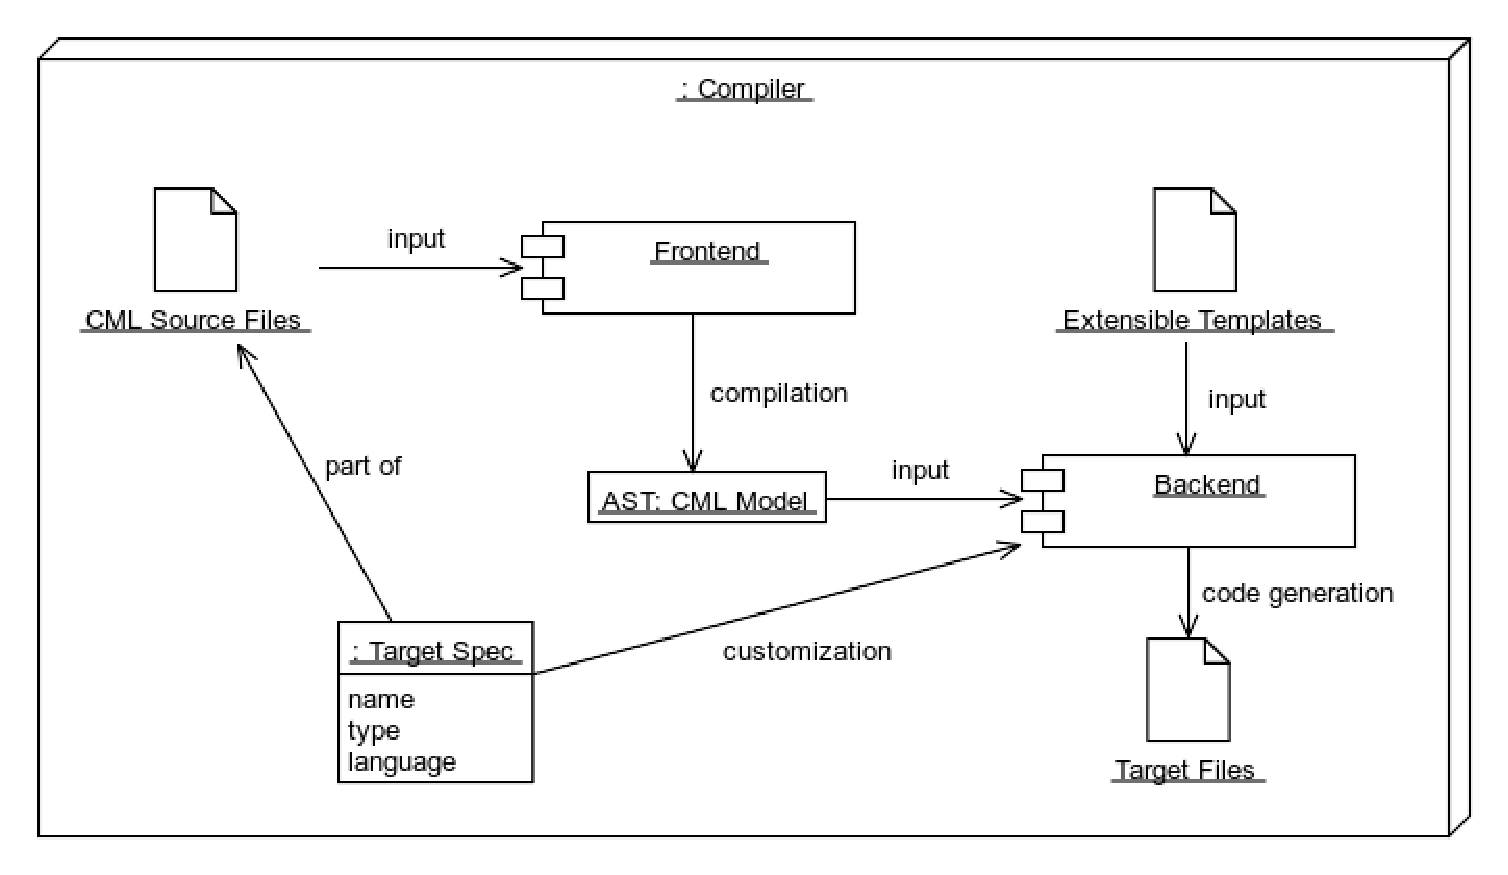
\includegraphics[width=\textwidth]{compiler/figure-overview}
\caption{An architectural overview of the CML compiler.}
\label{fig:overview}
\end{figure}

The CML compiler's overall architecture follows the standard compiler design literature \cite{torben}. An overview diagram of the architecture is shown in figure \ref{fig:overview}.
The two main components of the compiler,
and the artifacts they work with,
are presented in the next subsections.


    \section[The Frontend]{The Compiler Frontend}
    \label{sec:frontend}
    The frontend receives as input the \emph{CML source files}.
It will parse the files and generate an internal representation of the \emph{CML model}.

Syntactical and semantic validations will be performed at this point.
Any syntax and constraint errors are presented to the developer, interrupting the progress to the next phase.
If the \emph{source files} are parsed and validated successfully, then the internal representation (the AST) of the \emph{CML model} is provided as the input for the \emph{backend} component.


    \section[The Backend]{The Compiler Backend}
    \label{sec:backend}
    The backend receives the \emph{CML model AST} as input.
Based on the \emph{target specification} provided by the AST, chooses which \emph{extensible templates} to use for code generation.
The \emph{target files} are then generated, and become available to be consumed by other tools. The \emph{task declaration} plays the key role of determining the kind of \emph{target} to be generated.

CML extensible templates are implemented in StringTemplate \cite{st}.  The CML compiler uses StringTemplate for two purposes:

\begin{itemize}
\item \emph{File names and directory structure:}
each type of target generated by the CML compiler requires a different directory structure.
The CML compiler expects each target type to define a template file named ``files.stg'' (also known as \emph{files template}),
which will contain the path of all files to be generated. The \emph{files template} may use information provided by the \emph{task declaration}
in order to determine the file/directory names.
\item \emph{File content generation:}
each file listed under the \emph{files template} will have a corresponding \emph{content template} that specifies how the file's content must be generated. The \emph{content template} will receive as input one root-level element of the CML model, which will provide information to generate the file's content.
Each type of top-level model element should have a corresponding \emph{content template}. Templates are described in \emph{Code Generation} part of this specification.
\end{itemize}


  \chapter{Specification and Notations}
  \label{ch:notations}
  The following chapters will specify every element of CML metamodel.
Each chapter starts with a definition, followed by: an example;
the specification of the concrete syntax;
and then presenting the abstract syntax,
and how to transform the concrete syntax into the abstract one.

Chapters may also have sections that specify sub-elements
of the top-level CML metamodel element being described in the chapter level.
Each sub-element is described under its section
using the same definition structure (detailed below)
that is used to define the top-level elements.

The definition of each CML metamodel element is stated in plain English
on a paraprah (such as this one)
starting with the ``\textbf{Definition.}'' heading.
If a correspondence exists to an element of
the Entity-Relationship (ER) \cite{er} metamodel,
or to an element of the Unified Modeling Language (UML) \cite{uml} metamodel,
it is provided.

\begin{examples}
For each metamodel element declaration in CML,
examples are provided on a paraprah (such as this one),
starting with the ``\textbf{Examples.}'' heading.
This type of paragraph refers to a \verb+verbatim+ figure
containing the examples, and describes them as needed.
The examples are provided for illustrative purposes only,
and they are \emph{not} intended to be normative.
They may be excerpts of larger CML source files,
and thus may not be successfully compiled on their own.
\end{examples}

\begin{concrete-syntax}
The concrete syntax of each CML metamodel element is described
on a paragraph (such as this one),
starting with the ``\textbf{Concrete Syntax.}'' heading.
This type of paragraph refers to a \verb+verbatim+ figure,
which contains the actual ANTLR \cite{antlr} grammar
specifying the syntax for the CML metamodel element in question,
and it must be considered normative.
The appendix \ref{apx:concrete-syntax} presents all the grammar rules
in a single listing.
\end{concrete-syntax}

\begin{abstract-syntax}
The abstract syntax of each CML metamodel element is described
on a paragraph (such as this one),
starting with the ``\textbf{Abstract Syntax.}'' heading.
This type of paragraph refers to two types of figure:
the first figure presents a class diagram
with the EMOF \cite{mof}-based metamodel
of the element being described;
the second figure specifies the transformation
from the concrete syntax into instances of the metamodel classes,
which are the nodes of the abstract syntax tree
(the intermediate representation described in section \ref{sec:compiler}).
The notation used to specify the transformations is presented
in the appendix \ref{apx:lsl}.
Both figures must be considered normative.
\end{abstract-syntax}

\begin{constraints}
The constraints of each CML metamodel element are described
on a paragraph (such as this one),
starting with the ``\textbf{Constraints.}'' heading.
This type of paragraph refers to a \verb+verbatim+ figure,
which contains the OCL \cite{ocl} invariants
(and its definitions)
of the CML metamodel element in question,
and it must be considered normative.
Each invariant has a name in the format \verb+inv_name+
so that it can be referred by the compiler's error messages
and users.
Derived properties may also be defined before the constraints
in order to simplify the constraint expressions.
The appendix \ref{apx:ocl} presents all the constraint rules
in a single listing.
\end{constraints}

All metamodel elements referred by one of the descriptions defined above
(definitions, examples, etc.)
are emphasized in \emph{italic}.
If the descriptions of a CML metamodel element refer to another CML metamodel element,
the corresponding chapter or section defining the other element
is provided in parenthesis, like so (\ref{sec:org}).

Some sections may not follow the structure defined above.
These normally provide additional semantic information in plain English,
which cannot be described using the notations presented above.


\part{Conceptual Modeling}

  \chapter{Concepts}
  \label{ch:concepts}
  A \emph{concept} in CML represents anything
that has a coherent, cohesive and relevant meaning in a domain.
In the ER \cite{er} metamodel,
it corresponds to an \emph{entity set} (or an \emph{entity type});
in UML \cite{uml},
to a \emph{class}.
The CML \emph{concept} differs, however, from the UML \emph{class},
because it has only \emph{properties} (\ref{sec:properties}),
while the UML \emph{class} may also have \emph{operations}.

\begin{examples}
Figure \ref{fig:ex:concepts} presents some examples of \emph{concepts} declared in CML.
As shown,
a \emph{concept} may have zero or more \emph{properties}
(\ref{sec:properties}),
and a \emph{property} may optionally declare a \emph{type}
(\ref{sec:primitive-types}, \ref{sec:collection-types}).
Also, as shown in the concept \textbf{EBook} of the example,
a \emph{concept} may specialize
(\ref{sec:generalization})
another \emph{concept}.
\end{examples}

\begin{figure}
\verbatimfont{\small}
\lstinputlisting[language=cml]{examples/concepts.cml}
\caption{Concept Examples}
\label{fig:ex:concepts}
\end{figure}

\begin{concrete-syntax}
Figure \ref{fig:stx:concept} specifies the syntax used
to declare a \emph{concept}.
The \textbf{concept} keyword is followed by a NAME.
Optionally, a list of other NAMEs may be enumerated,
referring to other \emph{concepts}
that are generalizations (\ref{sec:generalization}) of the declared \emph{concept}.
A list of \emph{properties} (\ref{sec:properties}) may be declared under the \textbf{concept} block.
And the \textbf{abstract} keyword may precede the \textbf{concept} keyword, making a \emph{concept} abstract (\ref{sec:abstract}).
\end{concrete-syntax}

\begin{figure}
\verbatimfont{\small}
\lstinputlisting[language=antlr]{grammar/Concepts.txt}
\caption{Concept Declaration Syntax}
\label{fig:stx:concept}
\end{figure}

\begin{abstract-syntax}
Figure \ref{fig:meta:concept} presents the \emph{concept} metamodel
in an EMOF \cite{mof} class diagram,
and figure \ref{fig:ast:concept} specifies
the \emph{concept} transformation
from its concrete syntax to its abstract syntax.
For each \emph{concept} parsed by the compiler,
an instance of the \emph{Concept} class will be created,
and its properties will be assigned
according to parsed information:

\begin{itemize}

\item \emph{name}:
assigned with the value of the terminal node NAME.

\item \emph{abstract}:
set to \emph{true} if the \textbf{abstract} keyword
is found before the \textbf{concept} keyword;
otherwise, set to \emph{false}.

\item \emph{elements}:
an \emph{ordered set} referencing all \emph{properties}
parsed in the \textbf{concept} block.

\item \emph{generalizations}:
an \emph{ordered set} referencing all \emph{concepts}
whose NAMEs were enumerated in the \emph{GeneralizationList}.

\end{itemize}
\end{abstract-syntax}

\begin{figure}
\centering
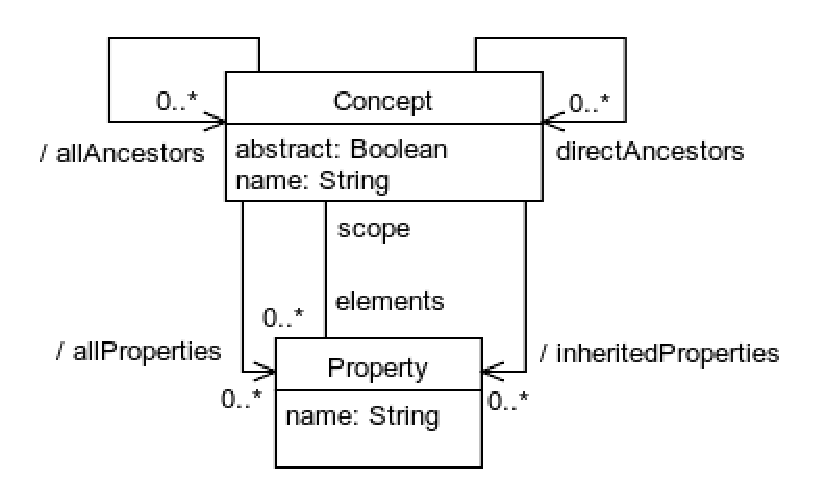
\includegraphics[width=0.5\textwidth]{metamodel/concept}
\caption{Concept Metamodel}
\label{fig:meta:concept}
\end{figure}

\begin{figure}
\verbatimfont{\small}
\lstinputlisting[language=lsl]{ast/concept.lsl}
\caption{Concept AST Instantiation}
\label{fig:ast:concept}
\end{figure}

\begin{constraints}
Figure \ref{fig:ocl:concept} presents the invariants of the \emph{concept} metamodel:

\begin{itemize}

\item \emph{unique\_concept\_name}:
Each \emph{concept} must have a unique NAME within its \emph{module} (\ref{ch:modules}).

\end{itemize}
\end{constraints}

\begin{figure}
\lstinputlisting[language=ocl_]{ocl/concept.ocl}
\caption{Concept Constraints}
\label{fig:ocl:concept}
\end{figure}


    \section{Example}
    Figure \ref{fig:ex:concepts} presents some examples of \emph{concepts} declared in CML.
As shown,
a \emph{concept} may have zero or more \emph{properties}
(\ref{ch:properties}),
and a \emph{property} may optionally declare a \emph{type}
(\ref{ch:primitive-types}, \ref{ch:sequence-types}).
Also, as shown in the concept \textbf{EBook} of the example,
a \emph{concept} may specialize
(\ref{ch:generalization})
another \emph{concept}.

\begin{figure}
\verbatimfont{\small}
\lstinputlisting[language=cml]{examples/concepts.cml}
\caption{Concept Examples}
\label{fig:ex:concepts}
\end{figure}


    \section{Syntax}
    Listing \ref{lst:stx:concept} specifies the syntax used
to declare a \emph{concept}.
The \textbf{concept} keyword is followed by a NAME.
Optionally, a list of other NAMEs may be enumerated,
referring to other \emph{concepts}
that are generalizations (\ref{ch:generalization}) of the declared \emph{concept}.
A list of \emph{properties} (\ref{ch:properties}) may be declared under the \textbf{concept} block.
And the \textbf{abstract} keyword may precede the \textbf{concept} keyword, making a \emph{concept} abstract (\ref{ch:abstract}).

\begin{code}
\verbatimfont{\small}
\lstinputlisting[language=antlr]{grammar/Concepts.txt}
\caption{Concept Concrete Syntax}
\label{lst:stx:concept}
\end{code}

Figure \ref{fig:meta:concept} presents the \emph{Concept} metaclass
in an EMOF \cite{mof} class diagram,
and listing \ref{lst:ast:concept} specifies
the \emph{concept} transformation
from its concrete syntax to its abstract syntax.
For each \emph{concept} parsed by the compiler,
an instance of the \emph{Concept} class will be created,
and its properties will be assigned
according to parsed information:

\begin{itemize}

\item \emph{name}:
assigned with the value of the terminal node NAME.

\item \emph{abstract}:
set to \emph{true} if the \textbf{abstract} keyword
is found before the \textbf{concept} keyword;
otherwise, set to \emph{false}.

\item \emph{elements}:
an \emph{ordered set} referencing all \emph{properties}
parsed in the \textbf{concept} block.

\item \emph{generalizations}:
an \emph{ordered set} referencing all \emph{concepts}
whose NAMEs were enumerated in the \emph{GeneralizationList}.

\end{itemize}

\begin{figure}
\centering
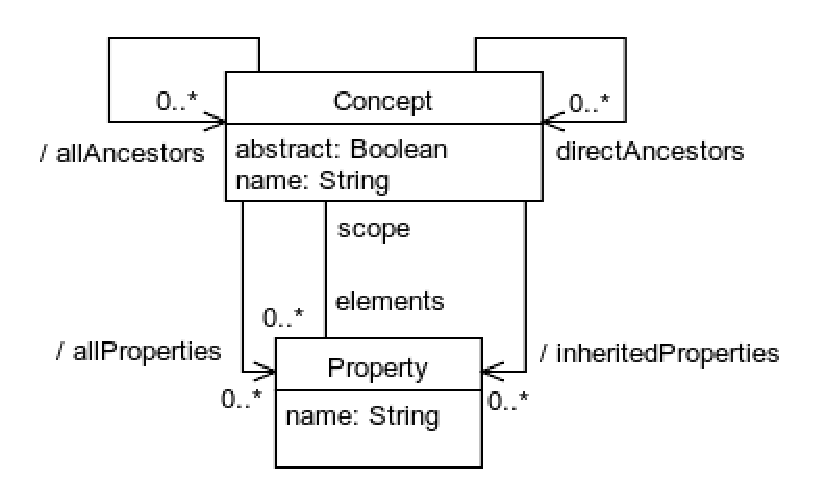
\includegraphics[width=0.5\textwidth]{metamodel/concept}
\caption{Concept Abstract Syntax}
\label{fig:meta:concept}
\end{figure}

\begin{code}
\verbatimfont{\small}
\lstinputlisting[language=lsl]{ast/concept.lsl}
\caption{Concept AST Instantiation}
\label{lst:ast:concept}
\end{code}


    \section{Model Validation}
    Listing \ref{lst:ocl:concept} presents the invariants of the \emph{Concept} metaclass:

\begin{itemize}

\item \emph{unique\_concept\_name}:
Each \emph{concept} must have a unique NAME within its \emph{module}.

\end{itemize}

\begin{code}
\lstinputlisting[language=ocl_]{ocl/concept.ocl}
\caption{Concept Constraints}
\label{lst:ocl:concept}
\end{code}


  \chapter{Properties}
  \label{ch:properties}
  A \emph{property} in CML may hold \emph{values} of \emph{primitive types} (\ref{ch:primitive-types}),
in which case they correspond to \emph{attributes} (\ref{ch:attributes})
on the ER \cite{er} and UML \cite{uml} metamodels.
Or they may hold references, or \emph{sequences} of references (\ref{ch:sequence-types}),
linking to instances of other \emph{concepts} (\ref{ch:concepts}),
in which case they correspond to a \emph{relationship} on the ER metamodel,
or to \emph{associations} (\ref{ch:associations}) on the UML metamodel.


    \section{Example}
    Figure \ref{fig:ex:properties} presents some examples of \emph{properties} declared in CML.
As shown in the examples,
a \emph{property} may be an \emph{attribute} (\ref{ch:attributes})
of a \emph{primitive type} (\ref{ch:primitive-types}),
or represent the role/end of an \emph{association} (\ref{ch:associations}).

\begin{figure}
\verbatimfont{\small}
\lstinputlisting[language=cml]{examples/properties.cml}
\caption{Property Examples}
\label{fig:ex:properties}
\end{figure}


    \section{Syntax}
    Listing \ref{lst:stx:property} specifies the syntax used
to declare a \emph{property}.
The NAME is followed by a \emph{typeDeclaration}
(\ref{ch:primitive-types}).
Optionally, an \emph{expression} (\ref{ch:expressions}) may be specified
in order to set the initial value.

\begin{code}
\verbatimfont{\small}
\lstinputlisting[language=antlr]{grammar/Properties.txt}
\caption{Property Concrete Syntax}
\label{lst:stx:property}
\end{code}

Figure \ref{fig:meta:concept} presents the \emph{Property} metaclass
in an EMOF \cite{mof} class diagram of the CML metamodel,
and listing \ref{lst:ast:property} specifies
the transformation
from the \emph{property} concrete syntax to its abstract syntax.
For each \emph{property} parsed by the compiler,
an instance of the \emph{Property} class will be created,
and its properties will be assigned
according to parsed information:

\begin{itemize}

\item \emph{name}:
assigned with the value of the terminal node NAME.

\item \emph{type}:
if \emph{typeDeclaration} is provided,
\emph{type} is set with the instance of the \emph{Type} class
matching the \emph{typeDeclaration}.

\item \emph{expression}:
if provided,
it contains the instance of the \emph{Expression} class
matching the parsed \emph{expression}.

\end{itemize}

\begin{code}
\verbatimfont{\small}
\lstinputlisting[language=lsl]{ast/property.lsl}
\caption{Property AST Instantiation}
\label{lst:ast:property}
\end{code}


    \section{Model Validation}
    Listing \ref{lst:ocl:property} presents the invariants
of the \emph{Property} metaclass:

\begin{itemize}

\item \emph{unique\_property\_name}:
Each \emph{property} must have a unique NAME within its \emph{concept}
(\ref{ch:concepts}).

\item \emph{property\_type\_specified\_or\_inferred}:
Either the \emph{property} explicitly defines a \emph{type}
or it defines an \emph{expression},
from which the type is inferred.
That is required for both regular, slot-based \emph{properties}
(which may provide an \emph{initialization expression})
and \emph{derived properties}
(which may have an \emph{expression} defining the derivation).

\item \emph{property\_type\_assignable\_from\_expression\_type}:
When both a \emph{type} and \emph{expression} are defined for a \emph{property},
the \emph{type} inferred from the \emph{expression} should be assignable to
the declared \emph{type}.
That is required for both regular, slot-based \emph{properties}
(which may provide an \emph{initialization expression})
and \emph{derived properties}
(which may have an \emph{expression} defining the derivation).

\end{itemize}

\begin{code}
\lstinputlisting[language=ocl_]{ocl/property.ocl}
\caption{Property Constraints}
\label{lst:ocl:property}
\end{code}


  \chapter{Attributes}
  \label{ch:attributes}
  In CML, \emph{attributes} are \emph{properties} (\ref{ch:properties})
of \emph{primitive types} (\ref{ch:primitive-types}).
They correspond to the \emph{Attribute} metaclass
in the ER \cite{er} metamodel;
in the UML \cite{uml} metamodel,
to the association \emph{attribute} between the metaclass \emph{Class}
and the metaclass \emph{Property}.

\emph{Attributes} serve as a \emph{slot} that holds a value of
the specified \emph{primitive type}.
An initial value may be specified as an \emph{expression} (\ref{ch:expressions}).
Some \emph{attributes}, however, may be continuosly
derive their \emph{value} from an \emph{expression} (not only initially),
in which case they are called \emph{derived attributes} (\ref{ch:derived-attributes}).

While initial values are only set when a \emph{concept} (\ref{ch:concepts})
is instantiated,
the value of \emph{derived attributes} is always evaluated
from the given \emph{expression},
and they cannot be set any other way.


    \section{Example}
    Listing \ref{lst:ex:attributes} presents some examples of \emph{attributes} declared in CML.
As shown,
the attribute \textbf{a} is a regular attribute definition 
that specifies the \emph{primitive type} (\ref{ch:primitive-types})
of the values that can be held by the \emph{attribute}'s slot.
The attribute \textbf{b} is an example showing how an \emph{attribute}
can be defined with an initial value.
As shown by the attribute \textbf{c}, 
an attribute may be derived from an \emph{expression}
that refers to other \emph{attributes}.
In order to differentiate \emph{attributes} with initial values
from \emph{derived attributes},
a forward slash (``/'') prefixes the name of the latter.
Attributes \textbf{d} and \textbf{e} are examples
where the type of the attribute,
instead of being specified,
is inferred from the given \emph{expression}.
Type inference is possible for both regular, slot-based \emph{attributes}
and \emph{derived attributes} that provide an \emph{expression}.

\begin{code}
\verbatimfont{\small}
\lstinputlisting[language=cml]{examples/attributes.cml}
\caption{Attribute Example}
\label{lst:ex:attributes}
\end{code}


    \section{Syntax}
    Figure \ref{fig:stx:property} specifies the syntax used
to declare any kind of \emph{property} (\ref{ch:properties}),
including \emph{attributes}.
The NAME of an \emph{attribute} is followed
by a \emph{typeDeclaration} of a \emph{primitive type}
(\ref{ch:primitive-types}).
Optionally, an \emph{expression} (\ref{ch:expressions}) may be specified
in order to set the initial value.
A \emph{derived attribute} must be prefixed with the forward-slash character,
as specified by DERIVED,
in which case the given \emph{expression} defines the value
of the \emph{attribute} at all times.

Since an \emph{attribute} in CML is just a \emph{property} (\ref{ch:properties})
with \emph{primitive types} (\ref{ch:primitive-types}),
the \emph{property} metaclass in the CML metamodel is used to represent
\emph{attributes}.
Figure \ref{fig:meta:property} presents the \emph{property} metaclass
in an EMOF \cite{mof} class diagram,
and figure \ref{fig:ast:property} specifies
the \emph{property} transformation
from its concrete syntax to its abstract syntax.


  \chapter{Derived Attributes}
  \label{ch:derived-attributes}
  A \emph{concept} in CML may have \emph{attributes} (\ref{ch:attributes})
that do not hold specific \emph{values},
but instead provide a \emph{value} derived from an \emph{expression} (\ref{ch:expressions}).
These are called \emph{derived attributes}.
Unlike an \emph{expression} used to initialize a \emph{non-derived attribute},
the \emph{expression} of a \emph{derived attribute} is evaluated
every time the \emph{value} of an \emph{attribute} is fetched.

In the UML \cite{uml} metamodel,
the \emph{Property} metaclass has a meta-attribute named \emph{isDerived},
which determines whether an \emph{attribute} is derived or not.
A \emph{derived attribute} in UML may be defined using a OCL \cite{ocl} constraint;
while CML has \emph{expressions} as part of the language.

The ER \cite{er} metamodel,
in its original form,
does not allow for the differentiation of \emph{derived attributes}
as part of an \emph{entity set},
but it is possible to define \emph{retrieval operations} whose 
results would equal to \emph{values} of \emph{derived properties} in CML.
It can be said, however, that ER,
by defining an \emph{attribute} as a function from the \emph{entity set}
to the \emph{value set},
does not prescribe that all \emph{attributes} are memory-based,
nor does it prevent the definition of an \emph{attribute} function 
as an \emph{expression}.

The CML metamodel and its syntax, on the other hand,
define whether an \emph{attribute} is memory-based (a \emph{non-derived attribute})
or it is derived from an \emph{expression} (a \emph{derived attribute}).


    \section{Example}
    Figure \ref{fig:ex:attributes} presents two examples of \emph{derived attributes}
declared in CML.
As shown,
the attribute \textbf{c} is derived from an \emph{expression}
that refers to other \emph{attributes}.
In order to differentiate \emph{attributes} with initial values,
such as \textbf{b},
from \emph{derived attributes},
such as \textbf{c},
a forward slash (``/'') prefixes the name of the latter.
The attribute \textbf{e} is an example of a \emph{derived attribute}
where the type is inferred from the given \emph{expression},
instead of being specified.


    \section{Syntax}
    Figure \ref{fig:stx:property} specifies the syntax used
to declare any kind of \emph{property} (\ref{ch:properties}),
including \emph{derived attributes}.
A \emph{derived attribute} must be prefixed with the forward-slash character,
as specified by DERIVED,
in which case the given \emph{expression} provides the value
of the \emph{attribute} every time it is fetched.

The \emph{property} metaclass in the CML metamodel is used to represent
\emph{attributes}.
Figure \ref{fig:meta:property} presents the \emph{property} metaclass
in an EMOF \cite{mof} class diagram,
and figure \ref{fig:ast:property} specifies
the \emph{property} transformation
from its concrete syntax to its abstract syntax.
The \emph{derived} property of the \emph{Property} metaclass
defines whether the \emph{attribute} is derived or not.


  \chapter{Associations}
  \label{ch:associations}
  In CML,
an \emph{association} represents a relation between two \emph{concepts} (\ref{ch:concepts}),
where a reference to an \emph{instance} of each \emph{concept} is found in every tuple that is part of the relation.
When \emph{concepts} have an \emph{association},
its \emph{instances} are linked in such way that
it is possible to access an \emph{instance} of one \emph{concept}
from an \emph{instance} of the other \emph{concept}.

The UML \cite{uml} metamodel has a metaclass named \emph{Association} that has \emph{Property} instances,
whose \emph{types} are the \emph{Class} instances that are part of the \emph{association}.
In UML, the name of each \emph{Property} instance in the \emph{Association} metaclass
is known as the \emph{role} of the corresponding \emph{Class} in the \emph{association}.

On the CML metamodel, on other hand,
the \emph{Association} metaclass is only needed
when it is necessary to define \emph{bidirectional associations}.
For \emph{unidirectional associations},
only a \emph{property} is defined in the source \emph{concept},
making its \emph{type} the target \emph{concept}.

On the ER \cite{er} metamodel,
each \emph{association} is known as a \emph{relationship set},
and each tuple in this set is called a \emph{relationship}.
Unlike CML and UML,
the tuples in a \emph{relationship set} of an ER model
can be queried directly,
and no notion of \emph{property} is required as part of the \emph{entity type}
in order to access those \emph{relationships}.

As it is case for \emph{attributes} (\ref{ch:attributes}),
\emph{associations} in CML can also be derived from other \emph{associations}
(just as well as in UML);
they are called \emph{derived associations} (\ref{sec:derived-associations}).

\begin{examples}
Figure \ref{fig:ex:associations} presents some examples of \emph{associations} declared in CML.
The concept \textbf{Vehicle} contains the property \textbf{driver},
which may optionally refer to an instance of \textbf{Employee},
meaning that a \textbf{driver} may or may not be assigned to a single \textbf{Vehicle}.
The concept \textbf{Vehicle} also has the property \textbf{owner},
which always refers to an instance of \textbf{Organization},
meaning that an \textbf{owner} must always be assigned to each instance of \textbf{Vehicle}. 
Similarly,
the concept \textbf{Employee} has the property \textbf{employer},
which must always be assigned to instance of \textbf{Organization}.
Just below the declaration of \textbf{Organization},
we observe an association named \textbf{Employment},
which enumerates two \emph{properties}:
the first is \textbf{employer} from the concept \textbf{Employee};
the second is \textbf{employees} from the concept \textbf{Organization}.
What this \emph{association} implies is a correspondence between these two properties.
Every time a reference to an instance of \textbf{Organization} is assigned to
the slot \textbf{employer} of an instance of \textbf{Employee},
a reference to this same instance of \textbf{Employee} must be assigned to
the slot \textbf{employees} of the \textbf{Organization} instance.
However,
since the \emph{type} of \textbf{employees}
in the concept \textbf{Organization}
is a sequence of \textbf{Employee} instances,
the reference to the instance of \textbf{Employee} will actually be added to the sequence,
along with the other instances already found in the sequence.
Thus, the association \textbf{Employment} actually characterizes a \emph{bidirectional association}.
The association \textbf{VehicleOwnership} is another example of a \emph{bidirectional association};
in this case,
between \textbf{Vehicle}'s \textbf{owner} property and \textbf{Organization}'s \textbf{fleet} property.
It can be noticed, though, 
in this second \emph{bidirectional association},
that the \emph{types} of the \emph{properties} are declared along with their names;
such a \emph{type} declaration,
in the \emph{association} declaration,
is optional in CML,
but must match the original \emph{property} declaration under the \emph{concept} declaration,
if present.
The \textbf{driver} property in the concept \textbf{Vehicle} is a different case,
since this \emph{property} does not participate in any \emph{association} declaration
in figure \ref{fig:ex:associations}.
That's because there is no corresponding \emph{property} in the concept \textbf{Employee}
representing the other end of the \emph{association}.
As such, the property \textbf{driver} is representing the source end of a \emph{unidirectional association}.
The property \textbf{drivers} in the concept \textbf{Organization} will be explained
in the section \ref{sec:derived-associations}.
\end{examples}

\begin{figure}
\verbatimfont{\small}
\lstinputlisting[language=cml]{examples/associations.cml}
\caption{Association Examples}
\label{fig:ex:associations}
\end{figure}

\begin{concrete-syntax}
Figure \ref{fig:stx:association} specifies the syntax used
to declare an \emph{association}.
The \textbf{association} keyword is followed by a NAME.
A list of \emph{association ends} are declared under the \textbf{association} block.
For each declaration of an \emph{association end},
The \textbf{conceptName} and \textbf{propertyName} are optionally followed by a \emph{typeDeclaration}.
\end{concrete-syntax}

\begin{figure}
\verbatimfont{\small}
\lstinputlisting[language=antlr]{grammar/Associations.txt}
\caption{Association Declaration Syntax}
\label{fig:stx:association}
\end{figure}

\begin{abstract-syntax}
Figure \ref{fig:meta:association} presents the \emph{Association} metaclass
in an EMOF \cite{mof} class diagram,
and figure \ref{fig:ast:association} specifies
the \emph{association} transformation
from its concrete syntax to its abstract syntax.
For each \emph{association} parsed by the compiler,
an instance of the \emph{Association} class will be created,
and its properties will be assigned
according to parsed information:

\begin{itemize}

\item \emph{name}:
assigned with the value of the terminal node NAME.

\item \emph{members}:
an \emph{ordered set} referencing all \emph{associationEnd}
instances parsed in the \textbf{association} block.

\end{itemize}
\end{abstract-syntax}

\begin{figure}
\verbatimfont{\small}
\lstinputlisting[language=lsl]{ast/association.lsl}
\caption{Association AST Instantiation}
\label{fig:ast:association}
\end{figure}

\begin{constraints}

\end{constraints}

    \section{Example}
    Listing \ref{lst:ex:associations} presents some examples of \emph{associations} declared in CML.
The concept \textbf{Vehicle} contains the property \textbf{driver},
which may optionally refer to an instance of \textbf{Employee},
meaning that a \textbf{driver} may or may not be assigned to a single \textbf{Vehicle}.
The concept \textbf{Vehicle} also has the property \textbf{owner},
which always refers to an instance of \textbf{Organization},
meaning that an \textbf{owner} must always be assigned to each instance of \textbf{Vehicle}.
Similarly,
the concept \textbf{Employee} has the property \textbf{employer},
which must always be assigned to an instance of \textbf{Organization}.

Just below the declaration of \textbf{Organization},
we observe an association named \textbf{Employment},
which enumerates two \emph{properties}:
the first is \textbf{employer} from the concept \textbf{Employee};
the second is \textbf{employees} from the concept \textbf{Organization}.
What this \emph{association} implies is a correspondence between these two properties.
Every time a reference to an instance of \textbf{Organization} is assigned to
the slot \textbf{employer} of an instance of \textbf{Employee},
a reference to this same instance of \textbf{Employee} must be assigned to
the slot \textbf{employees} of the \textbf{Organization} instance.
However,
since the \emph{type} of \textbf{employees}
in the concept \textbf{Organization}
is a sequence of \textbf{Employee} instances,
the reference to the instance of \textbf{Employee} will actually be appended to the sequence
being held by the slot \textbf{employees} of the concept \textbf{Organization},
and maintained along with the other \textbf{Employee} instances already found in the sequence.
Thus, the association \textbf{Employment} actually characterizes a \emph{bidirectional association}.

The association \textbf{VehicleOwnership} is another example of a \emph{bidirectional association};
in this case,
between \textbf{Vehicle}'s \textbf{owner} property and \textbf{Organization}'s \textbf{fleet} property.
It can be noticed, though,
in this second \emph{bidirectional association},
that the \emph{types} of the \emph{properties} are declared along with their names;
such a \emph{type} declaration,
in the \emph{association} declaration,
is optional in CML,
but must match the original \emph{property} declaration under the \emph{concept} declaration,
if present.

The \textbf{driver} property in the concept \textbf{Vehicle} is a different case,
since this \emph{property} does not participate in any \emph{association} declaration
on listing \ref{lst:ex:associations}.
That's because there is no corresponding \emph{property} in the concept \textbf{Employee}
representing the other end of the \emph{association}.
As such, the property \textbf{driver} is representing the source end of a \emph{unidirectional association}.

The property \textbf{drivers} in the concept \textbf{Organization}
is \emph{derived association} (\ref{ch:derived-associations}).

\begin{code}
\verbatimfont{\small}
\lstinputlisting[language=cml]{examples/associations.cml}
\caption{Association Example}
\label{lst:ex:associations}
\end{code}


    \section{Syntax}
    The concrete syntax used to declare an \emph{association} in CML
is specified by listing \ref{lst:stx:association}.
First, the \textbf{association} keyword is followed by a NAME.
Then, a list of \emph{association ends} are declared under the \textbf{association} block.
For each declaration of an \emph{association end},
The \textbf{conceptName} and \textbf{propertyName} are optionally followed by a \textbf{typeDeclaration}.

\begin{code}
\verbatimfont{\small}
\lstinputlisting[language=antlr]{grammar/Associations.txt}
\caption{Association Concrete Syntax}
\label{lst:stx:association}
\end{code}

The \emph{Association} metaclass is presented 
in the EMOF \cite{mof} class diagram of figure \ref{fig:meta:associations},
and its instantiation from the concrete syntax is specified by listing \ref{lst:ast:associations}.
For each parsed \emph{association},
an instance of the \emph{Association} metaclass will be created,
and its meta-properties will be assigned
according to parsed information:

\begin{itemize}

\item \emph{name}:
assigned with the value of the token NAME.

\item \emph{members}:
an \emph{ordered set} referencing all \emph{associationEnd}
instances parsed in the \textbf{association} block.

\end{itemize}

\begin{code}
\verbatimfont{\small}
\lstinputlisting[language=lsl]{ast/associations.lsl}
\caption{Association AST Instantiation}
\label{lst:ast:associations}
\end{code}


    \section{Model Validation}
    The invariants of the metaclasses \emph{Association} and \emph{AssociationEnd}
are specified by listing \ref{lst:inv:associations}:

\begin{itemize}

\item \emph{association\_end\_property\_found\_in\_model}:
Each \emph{association end} enumerated under an \emph{association}
must correspond to a \emph{property} of the same name under the specified \emph{concept}.

\item \emph{association\_end\_type\_matches\_property\_type}:
If a \emph{type} is specified for a given \emph{association end},
its \emph{name} and \emph{cardinality} must match the \emph{type}
of the corresponding \emph{property}.

\item \emph{association\_must\_have\_two\_association\_ends}:
An \emph{association} must have exaclty two \emph{association ends},
since only \emph{binary associations} are supported in CML.

\item \emph{association\_end\_types\_must\_match}:
The \emph{concept} of one \emph{association end} must correspond
to the \emph{type} of the \emph{property} of the other \emph{association end},
and vice-versa.

\end{itemize}

\begin{code}
\lstinputlisting[language=ocl_]{ocl/associations.ocl}
\caption{Association Constraints}
\label{lst:inv:associations}
\end{code}


    \section{Model Translation}
    The concrete syntax used to declare an \emph{association} in CML
is specified by listing \ref{lst:stx:association}.
First, the \textbf{association} keyword is followed by a NAME.
Then, a list of \emph{association ends} are declared under the \textbf{association} block.
For each declaration of an \emph{association end},
The \textbf{conceptName} and \textbf{propertyName} are optionally followed by a \textbf{typeDeclaration}.

\begin{code}
\verbatimfont{\small}
\lstinputlisting[language=antlr]{grammar/Associations.txt}
\caption{Association Concrete Syntax}
\label{lst:stx:association}
\end{code}

The \emph{Association} metaclass is presented 
in the EMOF \cite{mof} class diagram of figure \ref{fig:meta:associations},
and its instantiation from the concrete syntax is specified by listing \ref{lst:ast:associations}.
For each parsed \emph{association},
an instance of the \emph{Association} metaclass will be created,
and its meta-properties will be assigned
according to parsed information:

\begin{itemize}

\item \emph{name}:
assigned with the value of the token NAME.

\item \emph{members}:
an \emph{ordered set} referencing all \emph{associationEnd}
instances parsed in the \textbf{association} block.

\end{itemize}

\begin{code}
\verbatimfont{\small}
\lstinputlisting[language=lsl]{ast/associations.lsl}
\caption{Association AST Instantiation}
\label{lst:ast:associations}
\end{code}


  \chapter{Derived Associations}
  \label{ch:derived-associations}
  \emph{Derived associations} are declared by \emph{derived properties} (\ref{ch:properties}),
which associate a \emph{source-concept} to a \emph{target-concept}
via an \emph{expression} (\ref{ch:expressions}).
In order to obtain a reference to a \emph{target-concept} (\ref{ch:concepts}),
it is necessary to evaluate the \emph{expression} of the \emph{derived property}.
Among the possible \emph{sub-expressions}
that are part of the \emph{expression} of the \emph{derived association},
there are \emph{path expressions} (\ref{ch:paths}) of other \emph{associations},
which server as the base for the \emph{derived association}.


  \chapter{Generalization / Specialization}
  \label{ch:generalization}
  A \emph{concept} (\ref{ch:concepts}) in CML may be generalized by another \emph{concept}.
In other words, a \emph{concept} may be considered a specialization of another \emph{concept}.
Generalized \emph{concepts} have \emph{properties} (\ref{sec:properties})
that apply to a larger set of instances,
while specialized \emph{concepts} have \emph{properties}
that only apply to a subset of those instances.

In the UML \cite{uml} metamodel,
such generalization/specialization relationship between \emph{classes}
is known as \emph{generalization}, which is the name of the metaclass in the UML metamodel.
The original version of the ER \cite{er} metamodel lacked this kind of relationship
between \emph{entity types}.


    \section{Example}
    Figure \ref{fig:ex:generalization} presents some examples of
generalization/specialization relationships declared in CML.
As shown,
a \emph{concept} (\ref{ch:concepts}) may specialize zero or more other \emph{concepts}.
The latter are called the generalizations,
while the former is called the specialization.
A generalization, such as \textbf{Shape},
may define \emph{attributes} (\ref{ch:attributes}),
such as \textbf{color} and \textbf{area},
or also the \emph{roles} in \emph{unidirecional associations} (\ref{ch:associations}).
Both \emph{attributes} and \emph{roles} are \emph{properties} (\ref{ch:properties}) shared among all its specializations.
Some of these \emph{properties} may be redefined by the some of the specializations,
as it is the case with the \emph{area} property,
which is redefined by \textbf{Rectangle}, \textbf{Rhombus} and \textbf{Square}.
Some specializations may also define new \emph{properties},
such as \textbf{width} and \textbf{height} in \textbf{Rectangle},
which characterize only instances of this specialization.
A \emph{concept} may be a specialization of two or more other \emph{concepts},
as seen with \textbf{Square},
which specializes both \textbf{Rectangle} and \textbf{Rhombus},
and thus can redefine \emph{properties} of both generalizations.
If a \emph{property} has been defined by more than one generalization,
then it must be redefined by the specialization
in order to resolve the definition conflict,
which is the case with \textbf{area} in \textbf{Square}. 
If a redefinition suitable for both generalizations is unattainable,
it may be an indication that either the specialization or the generalizations
are unsound from the domain's prospective.

\begin{figure}
\verbatimfont{\small}
\lstinputlisting[language=cml]{examples/generalization.cml}
\caption{Generalization Examples}
\label{fig:ex:generalization}
\end{figure}


    \section{Syntax}
    Figure \ref{fig:stx:concept} specifies the syntax used
to declare a \emph{concept} (\ref{ch:concepts}),
and in turn its generalizations.
A list of NAMEs may be enumerated after the declared \emph{concept}'s NAME,
referring to other \emph{concepts} that this concept is a specialization of.

Figure \ref{fig:meta:concept} presents the \emph{Concept} metaclass
in an EMOF \cite{mof} class diagram of the CML metamodel,
and figure \ref{fig:ast:concept} specifies
the \emph{concept} transformation
from its concrete syntax to its abstract syntax.
There is a unidirecional association in the \emph{Concept} class
that keeps track of the generalization/specialization relationships,
which is named \emph{generalizations}.
It is an \emph{ordered set} referencing all \emph{concepts}
whose NAMEs were enumerated in the \emph{GeneralizationList}
of the declared \emph{concept}.


    \section{Model Validation}
    Figure \ref{fig:ocl:generalization} presents the invariants
of the \emph{Concept} and \emph{Property} classes
related to \emph{generalizations}:

\begin{itemize}

\item \emph{not\_own\_generalization}:
A \emph{concept} (\ref{ch:concepts}) may not be listed on its own \emph{GeneralizationList},
nor on the \emph{GeneralizationList} of its direct or indirect generalizations.

\item \emph{compatible\_generalizations}:
The \emph{generalizations} of a \emph{concept} must all be compatible between themselves,
that is, no two \emph{generalizations} may have a \emph{property} with the same name
but a different type.

\item \emph{generalization\_compatible\_redefinition}:
A \emph{property} may only be redefined with the same type defined in the \emph{generalizations}.

\item \emph{conflict\_redefinition}:
A \emph{concept} is required to redefine a \emph{property} that 
has been defined by two or more of its \emph{generalizations}
in order to resolve the definition conflict.
That is required only if the \emph{property} has been initialized or derived
in at least one of the \emph{generalizations}.
Otherwise, the redefinition is not required.

\end{itemize}

\begin{figure}
\lstinputlisting[language=ocl_]{ocl/generalization.ocl}
\caption{Generalization Constraints}
\label{fig:ocl:generalization}
\end{figure}


  \chapter{Abstractions}
  \label{ch:abstract}
  An \emph{abstraction} in CML is a \emph{concept} (\ref{ch:concepts})
that cannot create instances on its own,
but instead serves as a \emph{generalization} (\ref{ch:generalization})
for other \emph{concepts},
which in turn can create their own instances.
Thus, all instances of an \emph{abstraction}
are first instances of its \emph{specializations}.

In CML, an \emph{abstraction} may also define a \emph{derived property} (\ref{ch:properties})
without providing an \emph{expression} (\ref{ch:expressions}) in its definition;
such \emph{properties} are called \emph{abstract properties}.

CML's support for \emph{abstractions} matches UML's \cite{uml},
which allows the declaration of \emph{abstract classes}
by setting the \emph{isAbstract} attribute of a \emph{Class} instance to \emph{true}.
UML also allows the declaration of \emph{abstract attributes} and \emph{abstract operations}.

The original version of the ER \cite{er} metamodel, however,
as a consequence of lacking the \emph{generalization/specialization} relationship,
has not considered the notion of \emph{abstract entities}.


    \section{Example}
    Listing \ref{lst:ex:abstract} presents an example of an \emph{abstract concept} declared in CML.
As shown, the concept \textbf{Shape} is tagged as \emph{abstract},
and as such no direct instances of \emph{Shape} are ever instantiated.
As an \emph{abstract concept}, \textbf{Shape} can define \emph{abstract properties},
like \textbf{area}, which is just a \emph{derived property} (\ref{ch:properties})
without an \emph{expression} (\ref{ch:expressions}).
An \emph{abstract concept} may also define concrete \emph{properties},
such as \textbf{color} in \textbf{Shape}.
The concept \textbf{Circle} is a \emph{especialization} of \textbf{Shape}
that must redefine the property \textbf{area}
(and provide an \emph{expression})
if it is to be considered a \emph{concrete concept}.
As a \emph{concrete concept},
\textbf{Circle} may have direct instances,
which are in turn instances of \emph{Shape} as well.
\textbf{Circle} may also redefine \emph{concrete properties} of \textbf{Shape},
like \textbf{color},
but the redefinition is not a requirement in this case.
In \textbf{UnitCircle},
we can observe that the redefinition of an \emph{abstract property},
such as \textbf{area},
may be made \emph{concrete};
meaning it does not need to be redefined as a \emph{derived property}.
The converse situation is also allowed in CML,
where a \emph{concrete property} is redefined by as a \emph{derived property},
as illustrated with the property \textbf{radius} in \textbf{UnitCircle}.

\begin{code}
\verbatimfont{\small}
\lstinputlisting[language=cml]{examples/abstract.cml}
\caption{Abstract Concept Example}
\label{lst:ex:abstract}
\end{code}



    \section{Syntax}
    Listing \ref{lst:stx:concept} specifies the syntax used
to declare a \emph{concept} (\ref{ch:concepts}) in CML.
It shows that a \emph{concept} may be tagged with the \textbf{abstract} keyword
in order to convey it as an \emph{abstract concept}.
Listing \ref{lst:stx:property} specifies the syntax used
to declare a \emph{property} (\ref{ch:properties}) in CML.
It shows that a \emph{property} may be prefixed with a forward slash (``/'')
in order to mark it as a \emph{derived property}.
If the optional \textbf{expression} is not provided,
the property is then considered an \emph{abstract property}.

Figure \ref{fig:meta:concept} presents the \emph{concept} metamodel
in an EMOF \cite{mof} class diagram,
and listing \ref{lst:ast:concept} specifies
the \emph{concept} transformation
from its concrete syntax to its abstract syntax.
There is a \textbf{Boolean} attribute named \textbf{abstract} in the \emph{Concept} class
that determines whether a \emph{concept} is \emph{abstract} or not.


    \section{Model Validation}
    Listing \ref{lst:ocl:abstract} presents the invariants
of the \emph{Concept} and \emph{Property} classes in CML's EMOF \cite{mof} metamodel
related to \emph{abstract concepts}:

\begin{itemize}

\item \emph{abstract\_property\_redefinition}:
A \emph{concrete concept} must redefine concretely all \emph{abstract properties} of 
its \emph{generalizations}.

\item \emph{abstract\_property\_in\_abstract\_concept}:
Only \emph{abstract concepts} may have \emph{abstract properties}.

\end{itemize}

\begin{code}
\lstinputlisting[language=ocl_]{ocl/abstract.ocl}
\caption{Abstract Concept Constraints}
\label{lst:ocl:abstract}
\end{code}


\part{Expressions}

  \chapter{Expressions}
  \label{ch:expressions}
  An \emph{expression} in CML is used to compute
\emph{values} (\ref{ch:primitive-types}) and sequences (\ref{ch:sequence-types})
that initialize or derive \emph{properties} (\ref{ch:properties}).
On the UML \cite{uml} metamodel,
it corresponds to the \emph{Expression} metaclass;
in OCL \cite{ocl}, to \emph{OclExpressionCS}.

CML \emph{expressions} are designed to provide the same level of
expressivity provided by OCL \emph{expressions},
but the CML syntax varies from OCL's;
especially for OCL's \emph{collection operations},
which correspond to \emph{query expressions} (\ref{ch:queries}) in CML.



    \section{Examples}
    Listing \ref{lst:ex:expressions} has some examples of \emph{expressions} in CML.
As shown, there are different types of expressions:
\emph{literal values} (\ref{ch:literals}),
\emph{prefixed/infixed expressions}
(\ref{ch:arithmetic}, \ref{ch:logical}, \ref{ch:relational}, \ref{ch:referential},
\ref{ch:type-casting}, \ref{ch:type-casting}),
\emph{conditional expressions} (\ref{ch:conditionals}),
\emph{path expressions} (\ref{ch:paths})
and \emph{comprehension expressions} (\ref{ch:comprehensions}),
among others.

\begin{code}[H]
\verbatimfont{\small}
\lstinputlisting[language=cml]{examples/expressions.cml}
\caption{Expression Example}
\label{lst:ex:expressions}
\end{code}


    \section{Syntax}
    Listing \ref{lst:stx:expressions} specifies the syntax of all kinds of \emph{expressions} in CML.
It also lists them in their order of precedence.

Observe that the grammar in listing \ref{lst:stx:expressions} is ambiguous.
ANTLR \cite{antlr} resolves the ambiguity
based on the order in which the \emph{expression} alternatives are listed.
Thus, the order in listing \ref{lst:stx:expressions} defines
the precedence order among all \emph{operators} in CML.

Also, according to ANTLR,
and as required by CML,
all \emph{expressions} in the grammar are left-to-right associative,
except for the \emph{exponentiation expression},
which is right-to-left associative,
as defined by the \textbf{<assoc=right>} clause.

\begin{code}[H]
\verbatimfont{\small}
\lstinputlisting[language=antlr]{grammar/Expressions.txt}
\caption{Expression Syntax}
\label{lst:stx:expressions}
\end{code}


    \section{Metamodel}
    Figure \ref{fig:meta:expressions} displays the metamodel of
\emph{expressions} in CML.

\begin{figure}[H]
\centering
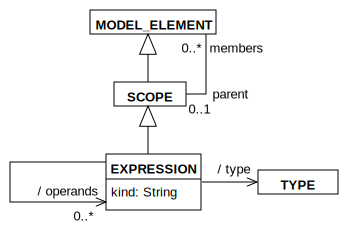
\includegraphics[width=0.7\textwidth]{metamodel/expressions}
\caption{Metamodel of Expressions}
\label{fig:meta:expressions}
\end{figure}


    \section{Model Synthesis}
    For each kind of \emph{expression} parsed by the compiler,
an instance of the \emph{Expression} metaclass is created,
and its properties are assigned
according to parsed information:

\begin{itemize}
  \item \emph{kind}:
  a \emph{String} value matching the \emph{Expression} subclass;
  for example, for the \emph{Literal} subclass, \textbf{kind = "literal"}.
  \item \emph{type}:
  a derived attribute that computes the \emph{Type} of the \emph{expression};
  each \emph{Expression} subclass will do its own \emph{Type} computation
  by providing its own definition for this derived attribute.
\end{itemize}


    \section{Model Validation}

    \section{Type Inference / Conformance}

    \section{Model Translation}

  \chapter{Literal Expressions}
  \label{ch:literals}
  For each one of the primitive types (\ref{ch:primitive-types}),
there are corresponding \emph{literal expressions}
that represent their values.
In CML, as it is the case with UML \cite{uml}, OCL \cite{ocl} and ER \cite{er},
each \emph{primitive type} may considered a mathematical \emph{set},
and a value allowed by a type corresponds to an \emph{element}
that belongs to this \emph{set}.

CML is able to infer the \emph{primitive type} of a \emph{property} (\ref{ch:properties})
based on the syntax of a \emph{literal expression}.
Each \emph{primitive type} in CML has a unique syntax.
In contrast,
OCL has the same \emph{literal} syntax for all \emph{numeric types},
and thus cannot infer a \emph{primitive type} from a \emph{literal expression}.


    \section{Examples}
    Table \ref{tab:literal-expr-examples} displays examples of \emph{literal expressions}
in CML.

\begin{table}[H]
\centering
\begin{tabular}
{ l l }
\hline
Type & Example \\
\hline
String & \verb+"Hello!\n"+ \\
Boolean & \verb!true! \\
Integer & \verb!123456! \\
Decimal & \verb!1234.567! \\
Byte & \verb!127b! \\
Short & \verb!1234s! \\
Long & \verb!1234567l! \\
Float & \verb!1234.567f! \\
Double & \verb!1234.567d!
\end{tabular}
\caption{Literal Expressions for Primitive Types}
\label{tab:literal-expr-examples}
\end{table}


    \section{Syntax}
    Table \ref{tab:literal-expr-syntax} displays the syntax of \emph{literal expressions}
in CML.

\begin{table}[H]
\centering
\begin{tabular}
{ l l }
\hline
Type & Syntax \\
\hline
String & \verb!'"' ('\\'[btnr"\\] | . )*? '"'! \\
Boolean & \verb!'true' | 'false'! \\
Integer & \verb!('0'..'9')+! \\
Decimal & \verb!('0'..'9')* '.' ('0'..'9')+! \\
Byte & \verb!('0'..'9')+ 'b'! \\
Short & \verb!('0'..'9')+ 's'! \\
Long & \verb!('0'..'9')+ 'l'! \\
Float & \verb!('0'..'9')* '.' ('0'..'9')+ 'f'! \\
Double & \verb!('0'..'9')* '.' ('0'..'9')+ 'd'!
\end{tabular}
\caption{Literal Expressions for Primitive Types}
\label{tab:literal-expr-syntax}
\end{table}


    \section{Metamodel}
    Figure \ref{fig:meta:literals} displays the metamodel of
\emph{literal expressions} in CML.

\begin{figure}[H]
\centering
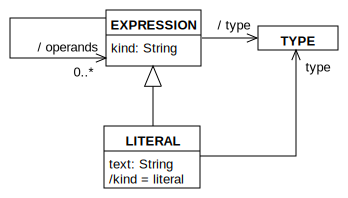
\includegraphics[width=0.7\textwidth]{metamodel/literals}
\caption{Metamodel of Literal Expressions}
\label{fig:meta:literals}
\end{figure}


    \section{Model Synthesis}

    \section{Model Validation}

    \section{Type Inference / Conformance}

    \section{Model Translation}

  \chapter{Arithmetic Expressions}
  \label{ch:arithmetic}
  \emph{Arithmetic expressions} are composed by
the \emph{arithmetic operators},
which only accept as operands
the \emph{expressions} of \emph{numeric} (\ref{ch:numeric-types})
and \emph{floating-point} (\ref{ch:floating-point}) types.


    \section{Examples}
    Table \ref{tab:arithmetic-examples} displays examples of \emph{arithmetic expressions}
in CML.

\begin{table}[H]
\centering
\begin{tabular}
{ l l l }
\hline
Operator & Operation & Example \\
\hline
\verb!^! & Exponentiation & \verb!3 ^ 2! \\
\verb!*!, \verb!/!, \verb!%! & Multiplication, Division, Modulo & \verb!6 * 2 / 3 % 4!  \\
\verb!+!, \verb!-! & Addition, Subtraction & \verb!6 + 2 - 1! \\
\end{tabular}
\caption{Examples using the Arithmetic Operators}
\label{tab:arithmetic-examples}
\end{table}


    \section{Syntax}
    Listing \ref{lst:stx:expressions} specifies the syntax of
the \emph{arithmetic expressions} in CML.
It also lists them in their order of precedence
in relation to other kinds of \emph{expressions}.


    \section{Metamodel}
    Figure \ref{fig:meta:arithmetic} displays the metamodel of
\emph{arithmetic expressions} in CML.

\begin{figure}[H]
\centering
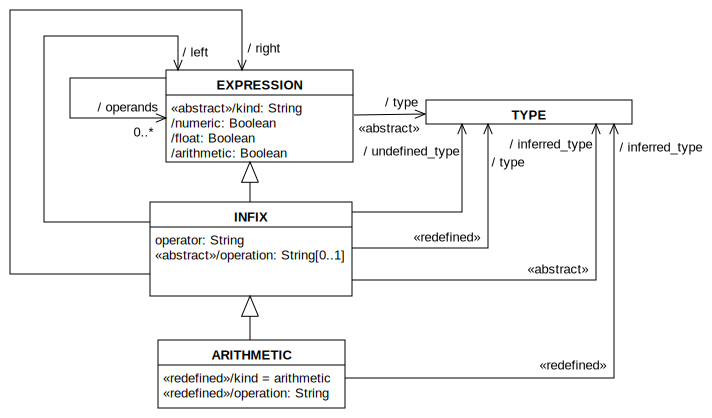
\includegraphics[width=1.2\textwidth]{metamodel/arithmetic}
\caption{Metamodel of Arithmetic Expressions}
\label{fig:meta:arithmetic}
\end{figure}


    \section{Model Synthesis}

    \section{Model Validation}
    Table \ref{tab:arithmetic-constraints} shows the precende order and associativity of \emph{arithmetic operators}
in CML.

\begin{table}[H]
\centering
\begin{tabular}
{ l l l }
\hline
Operator & Operation & Associativity \\
\hline
\verb!^! & Exponentiation & Right \\
\verb!*!, \verb!/!, \verb!%! & Multiplication, Division, Modulo & Left  \\
\verb!+!, \verb!-!$^*$ & Addition, Subtraction & Left \\
\multicolumn{3}{l}{\footnotesize{$^*$The addition/subtraction operators
may also be prefixed in the unary form.}}
\end{tabular}
\caption{Arithmetic Operators in Precedence Order}
\label{tab:arithmetic-constraints}
\end{table}

All \emph{arithmetic operators} are infixed,
but the addition (\verb|+|) and subtraction (\verb|-|) operators may also be prefixed when used in the unary form.
The associativity of the arithmetic operators is from left to right,
except for the exponentiation operator (\verb|^|),
where it is from right to left.

A validation error should reported by the compiler if any of the \emph{operands}
of an \emph{arithmetic expression} is inferred to be of a \emph{type}
other than \emph{numeric} (\ref{ch:numeric-types})
or \emph{floating-point} (\ref{ch:floating-point}).


    \section{Type Inference / Conformance}

    \section{Model Translation}

  \chapter{Logical Expressions}
  \label{ch:logical}
  \emph{Logical expressions} are composed by the \emph{logical operators},
which only accept as operands the \emph{expressions} (\ref{ch:expressions})
of the \emph{Boolean} type (\ref{ch:boolean}).


    \section{Examples}
    Table \ref{tab:logical-expr-examples} displays examples of
\emph{logical expressions} in CML.

\begin{table}[H]
\centering
\begin{tabular}
{ l l l }
\hline
Operator & Operation & Example \\
\hline
\verb!not! & Negation & \verb!not p! \\
\verb!and! & Conjunction & \verb!p and q! \\
\verb!or! & Disjunction & \verb!p or q! \\
\verb!xor! & Exclusive Disjunction & \verb!p xor q! \\
\verb!implies! & Implication & \verb!p implies q! \\
\end{tabular}
\caption{Logical Operators in Precedence Order}
\label{tab:logical-expr-examples}
\end{table}


    \section{Syntax}
    Listing \ref{lst:stx:expressions} specifies the syntax of
the \emph{logical expressions} in CML.
It also lists them in their order of precedence
in relation to other kinds of \emph{expressions}.


    \section{Metamodel}
    Figure \ref{fig:meta:logical-expr} displays the metamodel of
\emph{logical expressions} in CML.

\begin{figure}[H]
\centering
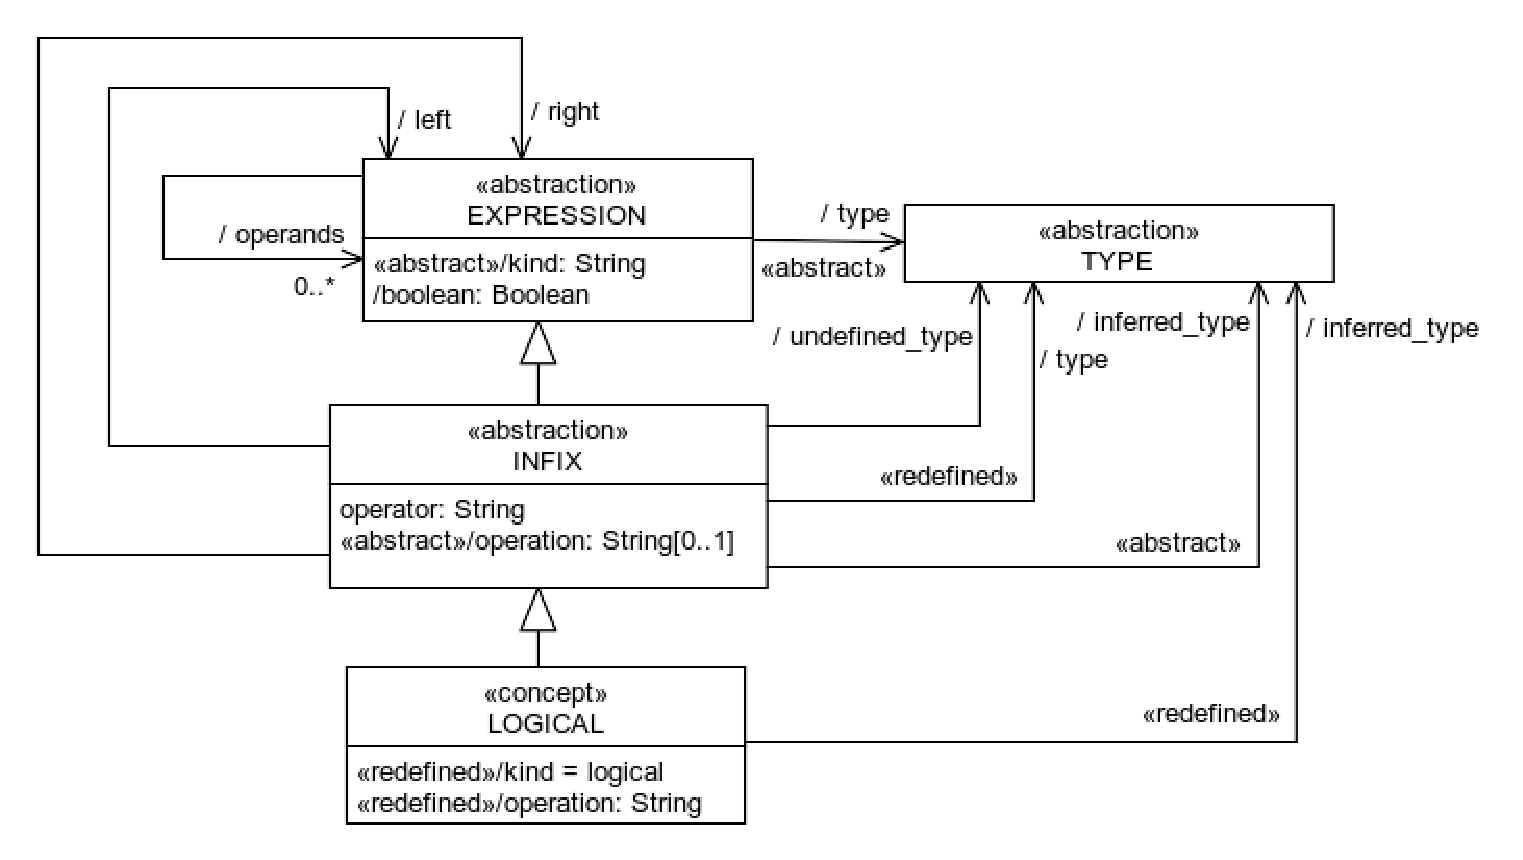
\includegraphics[width=1.2\textwidth]{metamodel/logical-expr}
\caption{Metamodel of Logical Expressions}
\label{fig:meta:logical-expr}
\end{figure}


    \section{Model Synthesis}

    \section{Model Validation}
    Table \ref{tab:logical-expr-constraints} shows
the precende order of the \emph{logical operators} in CML.

\begin{table}[H]
\centering
\begin{tabular}
{ l l }
\hline
Operator & Operation \\
\hline
\verb!not! & Negation \\
\verb!and! & Conjunction \\
\verb!or! & Disjunction \\
\verb!xor! & Exclusive Disjunction \\
\verb!implies! & Implication \\
\end{tabular}
\caption{Logical Operators in Precedence Order}
\label{tab:logical-expr-constraints}
\end{table}

All logical operators are infixed,
except for the negation operator (\verb|not|),
which is prefixed and unary.
The associativity of the binary operators is always from left to right.

A validation error should reported by the compiler if any of the \emph{operands}
of a \emph{logical expression} is inferred to be of a \emph{type}
other than \emph{Boolean}.


    \section{Type Inference / Conformance}

    \section{Model Translation}

  \chapter{Relational Expressions}
  \label{ch:relational}
  \emph{Relational expressions} are composed by the \emph{relational operators},
which only accept as operands the \emph{expressions} (\ref{ch:expressions})
of a \emph{relational type},
which include \emph{String} (\ref{ch:string}),
the \emph{numeric} (\ref{ch:numeric-types})
and \emph{floating-point} (\ref{ch:floating-point}) types,
but exclude \emph{Boolean} (\ref{ch:boolean})
and \emph{reference types} (\ref{ch:concept-types}).


    \section{Examples}
    Table \ref{tab:relational-expr-examples} shows
examples of the \emph{relational expressions} in CML.

\begin{table}[H]
\centering
\begin{tabular}
{ l l l }
\hline
Operators & Operation & Example \\
\hline
\verb!<!, \verb!<=!, \verb!>!, \verb!>=! & Ordering & \verb!3 < 2! \\
\verb!==!, \verb|!=| & Equality, Unequality & \verb|6 != 3|
\end{tabular}
\caption{Relational Operators}
\label{tab:relational-expr-examples}
\end{table}


    \section{Syntax}
    Listing \ref{lst:stx:expressions} specifies the syntax of
the \emph{relational expressions} in CML.
It also lists them in their order of precedence
in relation to other kinds of \emph{expressions}.


    \section{Metamodel}

    \section{Model Synthesis}

    \section{Model Validation}
    Table \ref{tab:relational-expr-constraints} shows
the precende order of the \emph{relational operators} in CML.

\begin{table}[H]
\centering
\begin{tabular}
{ l l }
\hline
Operators & Operation \\
\hline
\verb!<!, \verb!<=!, \verb!>!, \verb!>=! & Ordering \\
\verb!==!, \verb|!=| & Equality, Unequality
\end{tabular}
\caption{Relational Operators}
\label{tab:relational-expr-constraints}
\end{table}

All \emph{relational operators} are infixed.
There is no associativity between them.

A validation error should reported by the compiler if any of the \emph{operands}
of a \emph{relational expression} is inferred to be of a \emph{type}
other than \emph{String} (\ref{ch:string}),
\emph{numeric} (\ref{ch:numeric-types})
or \emph{floating-point} (\ref{ch:floating-point}).


    \section{Type Inference / Conformance}

    \section{Model Translation}

  \chapter{Referential Expressions}
  \label{ch:referential}
  In CML, \emph{referential expressions} are composed by the referential operators,
which only accept as operands the \emph{expressions} (\ref{ch:expressions})
resulting in references (\ref{ch:reference}).
That excludes all \emph{primitive types} (\ref{ch:primitive-types}).
All referential operators are infixed.
There is no associativity between the referential operators.

The table \ref{tab:referential-equality} presents
the \emph{referencial-equality operators}.

\begin{table}[htbp]
\centering
\begin{tabular}
{ L{1cm} L{3cm} L{4.5cm} l }
\hline
Oper. & Operation & Resulting Type & Example \\
\hline
\verb|===| & Referential Equality & Boolean & \verb|c1 === c2| \\
\verb|!==| & Referencial Inequality & Boolean & \verb|c1 !== c2| \\
\end{tabular}
\caption{Referential-Equality Operators}
\label{tab:referential-equality}
\end{table}

The \emph{referential equality operator} (\verb|is|)
results in the \verb|true| value
if both operands reference the same instance.
The \emph{referential inequality operator} (\verb|is|)
results in \verb|true| if the refecences do not point to the same instance.


    \section{Examples}
    Table \ref{tab:referential-expr-examples} shows
examples of \emph{referential expressions} in CML.

\begin{table}[H]
\centering
\begin{tabular}
{ l l l }
\hline
Operator & Operation & Example \\
\hline
\verb|===| & Referential Equality & \verb|product === book| \\
\verb|!==| & Referencial Inequality & \verb|product !== book| \\
\end{tabular}
\caption{Referential Operators}
\label{tab:referential-expr-examples}
\end{table}


    \section{Syntax}
    Listing \ref{lst:stx:expressions} specifies the syntax of
the \emph{referential expressions} in CML.
It also lists them in their order of precedence
in relation to other kinds of \emph{expressions}.


    \section{Metamodel}

    \section{Model Synthesis}

    \section{Model Validation}
    The \emph{referential operators} are infixed.
There is no associativity between them.

A validation error should reported by the compiler if any of the \emph{operands}
of a \emph{referential expression} is inferred to be of a \emph{type}
other than a \emph{reference type} (\ref{ch:concept-types}).


    \section{Type Inference / Conformance}

    \section{Model Translation}

  \chapter{Conditional Expressions}
  \label{ch:conditionals}
  In CML, \emph{conditional expressions} allow alternating between
one or more \emph{expressions} (\ref{ch:expressions})
based on some \emph{condition},
which is an \emph{expression} of \emph{Boolean} type (\ref{ch:boolean}).
The remaining operands of a \emph{conditional expression}
-- the alternating \emph{expressions} --
may be of any type (\ref{ch:types}),
including the \emph{primitive types} (\ref{ch:primitive-types})
and \emph{references} (\ref{ch:concept-types}).

The \emph{conditional expressions} are divided in three categories:

\begin{itemize}
\item unary: only evaluates a single \emph{expression}
if the \emph{condition} evaluates to \verb!true!.
\item binary: results in the evaluation of the first \emph{expression}
if the \emph{condition} evaluates to \verb!true!;
otherwise, it results in the evaluation of the second \emph{expression}.
\item optional: the \emph{condition} is implicit;
it results in the first \emph{expression} if it provides a value;
else, it results in the second \emph{expression} if it provides a value;
otherwise, it results in \emph{none}.
\end{itemize}

The resulting type of a \emph{conditional expression}
is based on the type of its \emph{operands}.
The cardinality is also based on the \emph{operands}.


    \section{Examples}
    Table \ref{tab:conditional-expr-examples} displays examples of
\emph{conditional expressions} in CML.

\begin{table}[H]
\centering
\begin{tabular}
{ l l }
\hline
Expression & Example \\
\hline
\\
unary if & \verb|10 if i > 2| \\
unary unless & \verb|10 unless i <= 2| \\
\\
binary if-then-else & \verb|if i > 2 then 10 else 5| \\
binary if-else & \verb|10 if i > 2 else 5| \\
\\
conditional or & \verb|item.book or? item.accessory| \\
conditional xor & \verb|item.book xor? item.accessory| \\
\end{tabular}
\caption{Conditional Expressions}
\label{tab:conditional-expr-examples}
\end{table}


    \section{Syntax}
    Listing \ref{lst:stx:expressions} specifies the syntax of
the \emph{conditional expressions} in CML.
The table \ref{tab:conditional-expr-syntax} is another representation of the syntax.

\begin{table}[H]
\centering
\begin{tabular}
{ l l }
\hline
Expression & Example \\
\hline
\\
unary given & \verb|<expr> given <cond>| \\
unary unless & \verb|<expr> unless <cond>| \\
\\
binary if-then-else & \verb|if <cond>| \verb|then <expr1>| \verb|else <expr2>| \\
\\
conditional or & \verb|<expr1> or? <expr2>| \\
conditional xor & \verb|<expr1> xor? <expr2>| \\
\end{tabular}
\caption{Syntax of Conditional Expressions}
\label{tab:conditional-expr-syntax}
\end{table}


    \section{Metamodel}

    \section{Model Synthesis}

    \section{Model Validation}
    In \emph{conditional expressions},
the \emph{condition} must be of \emph{Boolean} type,
and the \emph{alternatives} must be of compatible types.


    \section{Type Inference / Conformance}

    \section{Model Translation}

  \chapter{Type Checking}
  \label{ch:type-checking}
  
The \emph{type-checking operator} (\verb|is|)
results in the \verb|true| value
if the instance referenced by the first operand
is of the \emph{type} (\ref{ch:types}) specified by the second operand,
or it is an \emph{specialization} of such type.
The \emph{nagative type-checking operator} (\verb|is|)
results in \verb|true| if the \emph{type} does not match.


    \section{Examples}
    The table \ref{tab:type-checking-examples} shows examples of
the \emph{type-checking expressions}.

\begin{table}[H]
\centering
\begin{tabular}
{ l l l }
\hline
Operator & Operation & Example \\
\hline
\verb|is| & Type-Checking & \verb|product is Book| \\
\verb|isnt| & Negative Type-Checking & \verb|product isnt Book| \\
\end{tabular}
\caption{Examples of Type-Checking Expressions}
\label{tab:type-checking-examples}
\end{table}


    \section{Syntax}
    Listing \ref{lst:stx:expressions} specifies the syntax of
the \emph{type-checking expressions} in CML.
It also lists them in their order of precedence
in relation to other kinds of \emph{expressions}.

The table \ref{tab:type-checking-syntax} is another representation of the syntax.

\begin{table}[H]
\centering
\begin{tabular}
{ l l l }
\hline
Operator & Operation & Syntax \\
\hline
\verb|is| & Type-Checking & \verb|<expr> is <typeDeclaration> | \\
\verb|isnt| & Negative Type-Checking & \verb|<expr> isnt <typeDeclaration>| \\
\end{tabular}
\caption{Syntax of Type-Checking Expressions}
\label{tab:type-checking-syntax}
\end{table}


    \section{Metamodel}

    \section{Model Synthesis}

    \section{Model Validation}

    \section{Type Inference / Conformance}

    \section{Model Translation}

  \chapter{Type Casting}
  \label{ch:type-casting}
  There are three \emph{type-casting operators} in CML.
The \emph{safe type-casting operator} (\verb|as|)
may only be applied when the casting is guaranteed to work
and the resulting expression has the same cardinality
as the original one.
The \emph{forced type-casting operator} (\verb|as!|)
may raise an exception at runtime
if the actual type of the instance is not compatible with the expected type.
The \emph{conditional type-casting operator} (\verb|as?|)
automatically selects the compatible instances,
never raising an expception at runtime.


    \section{Examples}
    The table \ref{tab:type-casting-examples} presents the \emph{type-casting expressions}.

\begin{table}[htbp]
\centering
\begin{tabular}
{ l l l }
\hline
Oper. & Operation & Example \\
\hline
\verb|as| & Safe Type-Casting & \verb|products as Book*| \\
\verb|as!| & Forced Type-Casting & \verb|products as! Book| \\
\verb|as?| & Condicional Type-Casting & \verb|products as? Book?|
\end{tabular}
\caption{Examples of Type-Casting Expressions}
\label{tab:type-casting-examples}
\end{table}


    \section{Syntax}
    The table \ref{tab:type-casting-syntax} shows the syntax of
the \emph{type-checking expressions}.

\begin{table}[H]
\centering
\begin{tabular}
{ l l l }
\hline
Operator & Operation & Syntax \\
\hline
\verb|as| & Safe Type-Casting & \verb|<expr> as <typeDeclaration>| \\
\verb|as!| & Forced Type-Casting & \verb|<expr> as! <typeDeclaration>| \\
\verb|as?| & Condicional Type-Casting & \verb|<expr> as? <typeDeclaration>|
\end{tabular}
\caption{Syntax of Type-Casting Expressions}
\label{tab:type-casting-syntax}
\end{table}


    \section{Metamodel}

    \section{Model Synthesis}

    \section{Model Validation}

    \section{Type Inference / Conformance}

    \section{Model Translation}

  \chapter{String Concatenation}
  \label{ch:string-concatenation}
  \emph{Expressions} (\ref{ch:expressions}) of the \emph{String} type (\ref{ch:string})
may be combined with the ampersand (\emph{\&}) operator
for concatenation (\ref{ch:string-concatenation}).
The resulting \emph{expression} is of \emph{String} type.

Only \emph{expressions} of \emph{primitive types} (\ref{ch:primitive-types})
may be used as operands of a \emph{string concatenation} expression.
In that case,
they are evaluated and the resulting value is converted to a \emph{String} value,
which is then concatenated like any other \emph{String} value.

The associativity of the concatenation operator is from left to right,
just like the \emph{arithmetic operators} (\ref{ch:arithmetic}).


    \section{Examples}
    Listing \ref{lst:ex:str-concat} presents an example of
a \emph{string concatenation expression} in CML.

\begin{code}[H]
\verbatimfont{\small}
\lstinputlisting[language=cml]{examples/str-concat.cml}
\caption{Example of String Concatenation}
\label{lst:ex:str-concat}
\end{code}


    \section{Syntax}
    Listing \ref{lst:stx:expressions} specifies the syntax of
the \emph{string concatenation expressions} in CML.
It also lists them in their order of precedence
in relation to other kinds of \emph{expressions}.


    \section{Metamodel}

    \section{Model Synthesis}

    \section{Model Validation}
    Only an \emph{expression} inferred to be of a \emph{primitive type} (\ref{ch:primitive-types})
may be used as an operand of a \emph{string concatenation} expression.
It is allowed that none of the operands are of \emph{String} type.
All operands are converted to \emph{String} before concatenation.

The associativity of the concatenation operator is from left to right,
just like the \emph{arithmetic operators} (\ref{ch:arithmetic}).


    \section{Type Inference / Conformance}
    The resulting \emph{expression} is always of the \emph{String} type,
regardless of the operand types.


    \section{Model Translation}
    The \emph{operands} are concatenated using the string concatenation operation
provided by the target language.
If the \emph{operand type} is not \emph{String},
then it is evaluated and the resulting value is converted to a \emph{String} value,
which is then concatenated with the other \emph{String} values.
The conversion of the \emph{operands} is dependent on the target programming language,
but it is normally done using the standard methods,
such as \emph{Objects.toString()} in Java, or \emph{str()} in Python.


  \chapter{Path Expressions}
  \label{ch:paths}
  In CML, \emph{path expressions} allow accessing
the \emph{values} (\ref{ch:primitive-types})
and \emph{references} (\ref{ch:references})
of \emph{properties} (\ref{ch:properties})
in instances of a \emph{concept} (\ref{ch:concepts}).
Be those \emph{properties}
the \emph{attributes} (\ref{ch:attributes})
or the \emph{association roles} (\ref{ch:associations})
of a \emph{concept} instance,
\emph{path expressions} will traverse through each \emph{property}
in the path in order to find the intended \emph{values} or \emph{references}.
They can also be applied to \emph{lambda parameters} (\ref{ch:lambdas}).


    \section{Examples}
    Listing \ref{lst:ex:paths} presents some examples of \emph{path expressions} in CML.

\begin{code}[H]
\verbatimfont{\small}
\lstinputlisting[language=cml]{examples/paths.cml}
\caption{Examples of Path Expressions}
\label{lst:ex:paths}
\end{code}


    \section{Syntax}
    Listing \ref{lst:stx:paths} specifies the syntax of
\emph{path expressions} in CML.

\begin{code}[H]
\verbatimfont{\small}
\lstinputlisting[language=antlr,firstline=47,lastline=48]{grammar/Expressions.txt}
\caption{Syntax of Path Expressions}
\label{lst:stx:paths}
\end{code}


    \section{Metamodel}

    \section{Model Synthesis}

    \section{Model Validation}

    \section{Type Inference / Conformance}

    \section{Model Translation}

  \chapter{Invocation Expressions}
  \label{ch:invocations}
  \emph{Invocations} apply a \emph{function} (\ref{ch:built-in-functions})
to some \emph{expressions} (\ref{ch:expressions})
-- the arguments --
that correspond to the \emph{function parameters}.
CML provides some \emph{built-in functions} in the base module.
New functions may be defined via
\emph{template functions} (\ref{ch:template-functions})
or via \emph{declared functions} (\ref{ch:declared-functions}).


    \section{Examples}
    Listing \ref{lst:ex:invocations} presents an example of
an \emph{invocation expression} in CML.

\begin{code}[H]
\verbatimfont{\small}
\lstinputlisting[language=cml]{examples/invocations.cml}
\caption{Invocation Example}
\label{lst:ex:invocations}
\end{code}


    \section{Syntax}
    Listing \ref{lst:stx:lambdas2} specifies the syntax of
\emph{invocation expressions} in CML.

\begin{code}[H]
\verbatimfont{\small}
\lstinputlisting[language=antlr,firstline=56,lastline=57]{grammar/Expressions.txt}
\caption{Syntax of Invocation Expressions}
\label{lst:stx:lambdas2}
\end{code}


    \section{Metamodel}

    \section{Model Synthesis}

    \section{Model Validation}

    \section{Type Inference / Conformance}

    \section{Model Translation}

  \chapter{Lambda Expressions}
  \label{ch:lambdas}
  CML allows the use of \emph{lambda expressions}
as an argument of the \emph{invocation} (\ref{ch:invocations})
of a \emph{function} (\ref{ch:built-in-functions}).
CML provides some \emph{built-in functions} in the \verb|cml_base| module
that accept a \emph{lambda expression} as an argument.


    \section{Examples}
    Listing \ref{lst:ex:lambdas} presents an example of
a \emph{lambda expression} in CML.

\begin{code}[H]
\verbatimfont{\small}
\lstinputlisting[language=cml]{examples/lambdas.cml}
\caption{Lambda Example}
\label{lst:ex:lambdas}
\end{code}


    \section{Syntax}
    Listing \ref{lst:stx:lambdas} specifies the syntax of
\emph{lambda expressions} in CML.

\begin{code}[H]
\verbatimfont{\small}
\lstinputlisting[language=antlr,firstline=50,lastline=54]{grammar/Expressions.txt}
\caption{Syntax of Lambda Expressions}
\label{lst:stx:lambdas}
\end{code}


    \section{Metamodel}

    \section{Model Synthesis}

    \section{Model Validation}

    \section{Type Inference / Conformance}

    \section{Model Translation}

  \chapter{Comprehension Expressions}
  \label{ch:comprehensions}
  CML supports a kind of \emph{expression} (\ref{ch:expressions})
called \emph{comprehension},
which is a flexible and expressive way
to create new \emph{sequences} (\ref{ch:sequence-types})
or to calculate \emph{values} or \emph{references} from existing ones.

The \emph{comprehension expressions} in CML are similar to the
set builder notation in mathematics,
and also to \emph{list comprehensions} in Python,
or \emph{for comprehensions} in Scala.
Unlike those languages, in CML,
\emph{comprehensions} can be combined using the pipe (\verb!|!) operator
and \emph{functions} (\ref{ch:comprehension-functions}),
making them more extensible.


    \section{Examples}
    Listing \ref{lst:ex:comprehensions} presents an example of
a \emph{comprehension expression} in CML.

\begin{code}[H]
\verbatimfont{\small}
\lstinputlisting[language=cml]{examples/comprehensions.cml}
\caption{Example of Comprehension Expression}
\label{lst:ex:comprehensions}
\end{code}


    \section{Syntax}
    Listing \ref{lst:stx:comprehensions} specifies the syntax of
\emph{comprehension expressions} in CML.

\begin{code}[H]
\verbatimfont{\small}
\lstinputlisting[language=antlr,firstline=59,lastline=71]{grammar/Expressions.txt}
\caption{Syntax of Comprehension Expressions}
\label{lst:stx:comprehensions}
\end{code}


    \section{Metamodel}

    \section{Model Synthesis}

    \section{Model Validation}

    \section{Type Inference / Conformance}

    \section{Model Translation}

\part{Functions}

  \chapter{Built-In Functions}
  \label{ch:built-in-functions}
  CML provides \emph{built-in functions} in the \verb|cml_base| module.
Most of them allow the processing of
references (\ref{ch:references}) and sequences (\ref{ch:sequence-types}).
Most are defined via template functions (\ref{ch:template-functions})
for each target programming language or technology.


  \chapter{Template Functions}
  \label{ch:template-functions}
  In CML, template functions (\ref{ch:template-functions})
allow the definition of a \emph{function} in the target programming language
via StringTemplate \cite{st}.
The declaration of a \emph{template function} only defines
the \emph{function signature},
while the \emph{function expression} is defined in StringTemplate
for each target programming language.


  \chapter{Declared Functions}
  \label{ch:declared-functions}
  In CML, \emph{functions} may be defined by a \emph{signature}
and a corresponding \emph{expression} (\ref{ch:expressions}).
The \emph{function signature} declares the \emph{parameter}
and the resulting \emph{type} (\ref{ch:types}).
Such a \emph{function} is translated to a target programming language
much like a \emph{derived attribute} (\ref{ch:derived-attributes}),
except that it does not belong to any particular \emph{concept} (\ref{ch:concepts})
and it may be invoked by any \emph{expression}, in any scope.

\emph{Functions} declared in CML are pure functions,
which means they have the following characteristics:

\begin{itemize}
\item they always evaluate to the same result given the same arguments;
\item their evaluation does not cause any side-effects or state mutation.
\end{itemize}

If a \emph{declared function} in its definition invokes other \emph{functions},
then those \emph{functions}
(being them other \emph{declared functions} or \emph{template functions} \ref{ch:template-functions})
must provide the same guarantees listed above in order
for the \emph{declared function} to be considered pure.


  \chapter{Comprehension Functions}
  \label{ch:comprehension-functions}
  Some \emph{functions},
being \emph{declared} (\ref{ch:declared-functions})
or just \emph{templates} (\ref{ch:template-functions}),
may be used in \emph{comprehension expressions} (\ref{ch:comprehension-functions})
if they have a specific \emph{signature}.
They may have one or more \emph{parameters}
as long as the first \emph{parameter} is named \verb|seq|
and it is of a \emph{sequence type} (\ref{ch:sequence-types}).


\part{Type System}

  \chapter{Types}
  \label{ch:types}
  CML is a statically-typed language.
All its \emph{properties} (\ref{ch:properties})
and \emph{expressions} (\ref{ch:expressions}) must have all their \emph{types} declared or inferred at compilation time.
Additionally:

\begin{itemize}
\item the type of a \emph{property} must be compatible with the type of its \emph{expression};
\item the type of the \emph{operands} must be compatible with its \emph{operator};
\item the type of a \emph{property redefinition} must be compatible with
the original \emph{property definition} in the \emph{generalization};
\item and the type of the arguments in a \emph{invocation} must be compatible with the
type of the declared parameters of the corresponding \emph{function}.
\end{itemize}

In order to verify the types during the model validation,
the model elements that have must have an associated type
are all specializations of the \emph{TypedElement} metaclass,
which has the abstract property \emph{type}.
Each \emph{TypedElement} specialization must redefine the \emph{type} property
in order to be able to infer its type.


  \chapter{Primitive Types}
  \label{ch:primitive-types}
  A \emph{primitive type} in CML is one of the pre-defined \emph{data types}
supported by the language,
as shown in tables \ref{tab:core-primitive-types} and \ref{tab:additional-primitive-types}.

In the ER \cite{er} metamodel,
a \emph{data type} is formally defined as a \emph{set} of \emph{values}
that can be held by an \emph{attribute} (\ref{ch:attributes}).
The original ER paper \cite{er} states that,
for each \emph{value set} (i.e. \emph{data type}),
there is a \emph{predicate} that can be used to test
whether a \emph{value} belongs to the \emph{set}.
In CML, instead,
\emph{literal expressions} are syntactically defined for each \emph{primitive type},
so that the \emph{type} can be inferred from the \emph{literal expression}.

On the original ER paper,
it is also said that \emph{values} in a \emph{value set}
may be equivalent to \emph{values} in another \emph{value set}.
In CML, also,
\emph{literal expressions} of the \emph{Integer} type may be equivalent
to \emph{literal expressions} of the \emph{Decimal},
and so with other \emph{numeric types}.
This allows \emph{expressions} (\ref{ch:expressions}) of a \emph{primitive type}
to be promoted to \emph{expressions} of another \emph{primitive type}
in order to allow \emph{type inference} of composite \emph{expressions}.

In the UML \cite{uml} metamodel,
there is a specific metaclass named \emph{PrimitiveType},
which matches to the same notion in CML.

\begin{table}[h]
\centering
\begin{tabular}
{l l l l l p{2cm} }
\hline
CML & Java & C\# & C++ & Python & TypeScript (JavaScript) \\
\hline
String & String & string & std::wstring & str & string \\
\multicolumn{6}{p{13cm}}{\footnotesize{16-bit Unicode character sequences.}} \\
\\
Boolean & boolean & bool & bool & bool & boolean \\
\multicolumn{6}{p{13cm}}{\footnotesize{Only values are the literal expressions: \textbf{true}, \textbf{false}.}}  \\
\\
Integer & int & int & int32\_t & int & number  \\
\multicolumn{6}{p{13cm}}{\footnotesize{32-bit signed two's complement integer.}}  \\
\\
Decimal* & BigDecimal & decimal & decimal128 & Decimal & number \\
\multicolumn{6}{p{13cm}}{\footnotesize{Arbitrary precision,
fixed-point,
or decimal floating-point,
depending on the target language.}} \\
\\
\multicolumn{6}{p{13cm}}{*The specification of Decimal type varies by target programming language.
Compared to the binary floating-point types (Float and Double),
the Decimal type is better suited for monetary calculations
at a performance cost.}
\end{tabular}
\caption{Core Primitive Types in CML.}
\label{tab:core-primitive-types}
\end{table}

\begin{table}[h]
\centering
\begin{tabular}
{l l l l l p{2cm} p{3.5cm} }
\hline
CML & Java & C\# & C++ & Python & TypeScript (JavaScript) & Specification \\
\hline
Byte & byte & byte & int8\_t & int & number & 8-bit signed two's complement integer \\
Short & short & short & int16\_t & int & number & 16-bit signed two's complement integer \\
Long & long & long & int64\_t & long & number & 64-bit signed two's complement integer \\
Float & float & float & float* & float & number & 32-bit IEEE 754 binary floating point \\
Double & double & double & double* & float & number & 64-bit IEEE 754 binary floating point \\
\\
\multicolumn{7}{p{12cm}}{*C++ floating point types may vary by hardware and compiler}
\end{tabular}
\caption{Additional Primitive Types in CML.}
\label{tab:additional-primitive-types}
\end{table}


    \section{Example}
    Figure \ref{fig:ex:primitive-types} presents examples
of \emph{atributes} declared with \emph{primitive types} in CML.
Each example corresponds to one of the \emph{primitive types}
supported by the language,
as shown in tables \ref{tab:core-primitive-types} and \ref{tab:additional-primitive-types}.
The \emph{target constructors}
of CML's base module will translate the primitive types to Java, C\#, C/C++,
Python, and TypeScript (JavaScript),
according to the mapping shown in the tables.

\begin{figure}
\verbatimfont{\small}
\lstinputlisting[language=cml]{examples/primitive_types.cml}
\caption{Example of \emph{Primitive Types}}
\label{fig:ex:primitive-types}
\end{figure}


    \section{Syntax}
    Figure \ref{fig:stx:type} specifies the syntax used
to declare any kind of \emph{type},
including \emph{primitive types}.
The NAME of the \emph{type} may be any of the \emph{primitive types}
defined in the column named \emph{CML}
of the tables \ref{tab:core-primitive-types} and \ref{tab:additional-primitive-types}.
Optionally, cardinality may also be specified
for a \emph{primitive type}.
The `*' cardinality suffix allows zero or more values to be stored
in a property as a collection type (\ref{sec:collection-types}).
The `?' cardinality suffix allows a single value to be stored, or none.
If no cardinality is specified,
a value must be assigned to the \emph{attribute}
when its \emph{concept} is instantiated.

\begin{figure}
\verbatimfont{\small}
\lstinputlisting[language=antlr]{grammar/Types.txt}
\caption{Type Declaration Syntax}
\label{fig:stx:type}
\end{figure}

Figure \ref{fig:meta:property} presents the \emph{Type} metaclass
in an EMOF \cite{mof} class diagram of the CML metamodel,
and figure \ref{fig:ast:type} specifies
the transformation
from the \emph{type} concrete syntax to its abstract syntax.

\begin{figure}
\verbatimfont{\small}
\lstinputlisting[language=lsl]{ast/type.lsl}
\caption{Type AST Instantiation}
\label{fig:ast:type}
\end{figure}


  \chapter{Boolean Type}
  \label{ch:boolean}
  The \emph{Boolean} type accepts only two literal expressions (\ref{ch:literals}): \verb|true| or \verb|false|.
When either of these two literals is found in \emph{expressions} (\ref{ch:expressions}),
its \emph{type} is inferred to be \emph{Boolean}.

Any \emph{expression} of the \emph{Boolean} type
may be used as an operand of \emph{logical expressions} (\ref{ch:logical}).


  \chapter{Numeric Types}
  \label{ch:numeric-types}
  From the smallest set to the largest one,
the \emph{numeric types} are the following in CML:
\emph{Byte}, \emph{Short}, \emph{Integer}, \emph{Long} and \emph{Decimal}.
They belong to the group of \emph{primitive types} (\ref{ch:primitive-types}),
which are shown in tables \ref{tab:core-primitive-types} and \ref{tab:additional-primitive-types}.


  \chapter{Floating-Point Types}
  \label{ch:floating-point}
  The \emph{floating-point types} in CML are \emph{Float} and \emph{Double}
for single-precision (32-bit) and double-precision (64-bit), respecitvely.
They belong to the group of \emph{primitive types} (\ref{ch:primitive-types}),
which are shown in tables \ref{tab:core-primitive-types} and \ref{tab:additional-primitive-types}.

There is a specific \emph{literal expression syntax} (\ref{ch:literals})
for each \emph{floating-point type},
which allows them to be inferred uniquely.
\emph{Literal expressions} of the \emph{Float} type may be equivalent
to \emph{literal expressions} within the same range of the \emph{Double} type.
This allows type inference of \emph{arithmetic expressions} (\ref{ch:arithmetic})
and \emph{relational expressions} (\ref{ch:relational}).
However,
in order to prevent data/precision loss,
it is not allowed the coercion of a value of a \emph{numeric type}
(\ref{ch:numeric-types}) to a value of a \emph{floating-point type},
and vice-versa.
That means it is not possible to combine \emph{expressions} (\ref{ch:expressions})
of \emph{floating-point} and \emph{numeric} types.


  \chapter{String Type}
  \label{ch:string}
  The \emph{String} type in CML represents a 16-bit Unicode character sequence,
matching the same type in other programming languages,
as described in table \ref{tab:core-primitive-types}.

There is a specific \emph{literal expression syntax} (\ref{ch:literals})
for \emph{String} values,
which allows them to be inferred uniquely.
\emph{Expressions} (\ref{ch:expressions}) of the \emph{String} type
may be the operands of \emph{relational expressions} (\ref{ch:relational}).
They may also be combined with the ampersand (\emph{\&}) operator
for concatenation (\ref{ch:string-concatenation}),
in which case the resulting \emph{expression} is of \emph{String} type.


  \chapter{Reference Types}
  \label{ch:concept-types}
  In CML, all \emph{type declarations}
referring to the name of a \emph{concept} (\ref{ch:concepts})
are instances of the \emph{ReferenceType} metaclass (\ref{ch:types});
in short, the \emph{type declaration} declares a \emph{reference type}.
A \emph{property} (\ref{ch:properties}) of a concept A,
whose type is declared or inferred to be of a concept B,
holds a reference to an instance of concept B; not the actual instance.
This allows the \emph{properties} of a concept C
to also reference the same instance of B.

Models in CML do not to keep track of the memory used
to store the actual instances.
CML expects the target programming language or technology
to support some kind of reference management,
such as a garbage collector in Java or automatic reference counting in Swift,
or still a database.
CML does not require any particular implementation.

The \emph{path expressions} (\ref{ch:paths})
whose result is of a \emph{reference type} may be used
in \emph{referential expressions} (\ref{ch:referential}),
\emph{type-checking expressions} (\ref{tab:type-checking}),
\emph{type-casting expressions} (\ref{tab:type-casting})
and in \emph{invocations} (\ref{ch:invocations}).


  \chapter{Tuple Types}
  \label{ch:tuple-types}
  \emph{Tuples} may be declared as the \emph{type} of
an \emph{argument} or the \emph{result} of a \emph{function} (\ref{ch:built-in-functions}).
A \emph{type declaration} that declares a \emph{tuple}
is an instance of the \emph{TupleType} metaclass.


  \chapter{Function Types}
  \label{ch:function-types}
  A \emph{function type declaration}
may used in \emph{functions} (\ref{ch:built-in-functions})
to declare that an \emph{argument} accepts a \emph{lambda expression} (\ref{ch:lambdas}).


\part{Code Generation}

  \chapter{Templates}
  \label{sec:templates}

  \chapter{Constructors}
  \label{sec:constructors}

  \chapter{Tasks}
  \label{sec:tasks}

  \chapter{Targets}
  \label{sec:targets}

\part{Organization and Sharing}

  \chapter{Modules}
  \label{ch:modules}

  \chapter{Libraries}
  \label{ch:libraries}

\part{Appendices}

\appendix

  \chapter{CML Concrete Syntax (Grammar)}
  \label{apx:concrete-syntax}
  \clearpage
\section{ANTLR Grammar}

\begin{framed}
\verbatimfont{\small}
\begin{verbatim}
// Compilation Units:
\end{verbatim}
\verbatiminput{grammar/CompilationUnits.txt}
\begin{verbatim}
// Concept Declarations:
\end{verbatim}
\verbatiminput{grammar/Concepts.txt}
\begin{verbatim}
// Property Declarations:
\end{verbatim}
\verbatiminput{grammar/Properties.txt}
\begin{verbatim}
// Type Declarations:
\end{verbatim}
\verbatiminput{grammar/Types.txt}
\begin{verbatim}
// Target Declarations:
\end{verbatim}
\verbatiminput{grammar/Targets.txt}
\begin{verbatim}
// Names:
\end{verbatim}
\verbatiminput{grammar/Names.txt}
\begin{verbatim}
// Literals:
\end{verbatim}
\verbatiminput{grammar/Literals.txt}
\verbatiminput{grammar/Ignored.txt}
\end{framed}


  \chapter{CML Abstract Syntax (Metamodel)}
  \label{apx:abstract-syntax}
  \input{metamodel.tex}

  \chapter{CML Abstract Syntax Tree (Instantiation)}
  \label{apx:ast}
  \input{ast.tex}

  \chapter{CML Constraints (Model Validation)}
  \label{apx:ocl}
  \clearpage

\begin{framed}
\verbatimfont{\small}
\verbatiminput{ocl/concept.ocl}
\verbatiminput{ocl/property.ocl}
\end{framed}


  \chapter{Language Specification Notation}
  \label{apx:lsl}
  \input{lsl.tex}

\backmatter

\bibliographystyle{plain}
\bibliography{references}

\end{document}
